%%%%%%%%%%%%%%%%%%%%%%%%%%%%%%%%%%%%%%%%%%%%%%%%%%%%%%%%%%%%%%%%%%%%%%%%%%%%%%
%
% Vorlage für eine Studien- oder Diplomarbeit für den Fachbereich Informatik
% der Universität Karlsruhe (TH)
%
% Autor:   Tilo Gockel
% Version: 0.920
% Datum:   12. Mai 2010
%
% Kontakt: Hochschule Aschaffenburg,
% Tilo Gockel (Dr.-Ing.), Forschungsreferat
%
% info@formbuch.de
% http://www.formbuch.de
%
% Anmerkungen
%
% 1.) article-Style, statt report-Style
%
% Soll statt des report-Styles der article-Style genutzt werden,
% so müssen chapters durch sections, sections durch subsection usw. ersetzt
% werden. Weiterhin kann ein Kapitelbeginn auf der rechten Seite dann nicht
% mehr durch openright eingestellt werden, nur noch durch jeweilige
% \cleardoublepage -Befehle (vgl. unten).
%
%
% 2.) Lizenz
%
% Das Template darf angepasst, verändert, erweitert und auch kommerziell vertrieben werden. 
% Die einzige Auflage ist, dass die Quelle des Templates in den Literaturquellen genannt 
% und im Text als Quelle referenziert wird. Hierzu ist dem Text ein kurzer Satz beizufügen, 
% und am Ende ist die Quelle einzufügen:
% Einzufügende Textzeile (Fußnote):
% Der vorliegende Text ist auf Basis des Latex-Templates zu [1] erstellt.
% Einzufügende zugehörige Quelle:
% [1] T. \mbox{Gockel}. Form der wissenschaftlichen Ausarbeitung. Springer-Verlag, Heidelberg, 2008. 
% Begleitende Materialien unter 
% \url$<http://wwwiaim.ira.uka.de/form-der-wissenschaftlichen-ausarbeitung>$.
% Weiterhin ist es sinnvoll, bei der Weitergabe des Templates die Latex-Quellen und die PDF-Datei
% nicht zu trennen.
%
%
% 3.) Versionsnummern der verwendeten Programme (alles unter Windows)
%
% (im Regelfall werden neuere Versionen aber eher von Vorteil sein)
%
%     Miktex 2.8
%     http://www.miktex.org
%
%     TexnicCenter Version 1.0 Stable Release Candidate 1
%     http://www.texniccenter.org
%
%     Texaide 4.0a
%     http://www.dessci.com/en/products/texaide
%
%     Adobe Acrobat Prof. 7.0
%     http://www.adobe.com/de/
%
%     Ghostscript 8.14, Ghostview 4.6
%     http://pages.cs.wisc.edu/~ghost
%
%     MS Office 2002, 2007 ...
%     http://office.microsoft.com/de-de/default.aspx
%
%     Adobe Photoshop CS4
%     http://www.adobe.com/de/products/photoshop/family/
%
%     Gnuplot 4.2
%     http://www.gnuplot.info
%   
%     PrettyPrinter a2ps
%     http://www.gnu.org/software/a2ps
%
%     Text-Ersetzungswerkzeug grep, unter Windows
%     http://gnuwin32.sourceforge.net/packages/grep.htm
%
%
%%%%%%%%%%%%%%%%%%%%%%%%%%%%%%%%%%%%%%%%%%%%%%%%%%%%%%%%%%%%%%%%%%%%%%%%%%%%%%
\documentclass[a4paper,english,twoside,openright,11pt]{report}



\usepackage[utf8]{inputenc} % Zeichensatz, ermöglicht die direkte Eingabe von Umlauten im Editor
\usepackage{ifpdf}
\ifpdf
    \usepackage[pdftex]{graphicx}
\else
     \usepackage[dvips]{graphicx}
\fi
\usepackage{float}            % bietet Option [H] für bombenfestes Verankern
%\usepackage[ngerman]{babel}   % Silbentrennung nach der neuen deutschen Rechtschreibung, z.B.: Sys-tem
\usepackage[english]{babel}   % Silbentrennung nach der neuen deutschen Rechtschreibung, z.B.: Sys-tem
\usepackage{amstext}          % für Klartext via \text{} in Formeln
\usepackage{amsfonts}         % für komplexere Formeln (Mengensymbole ...)
\usepackage{amssymb}          % für komplexere Formeln (Mengensymbole ...)
\usepackage{amsmath}              % für die Ausrichtung
\usepackage{bm}               % bold math, für \bm{}
\usepackage{enumerate}        % verbessert Aufzählungen
\usepackage[bottom]{footmisc} % Fussnoten am Seitenende
\usepackage{array}            % für Tabellen: bindet tabular-Umgebung ein
\usepackage{algorithm}        % für Algorithmen
\usepackage{algorithmic}      % für Algorithmen
\usepackage{ntheorem}
\usepackage{theorem}
\usepackage{pdfpages}         % für die Einbindung kompletter pdf-*Seiten*
\usepackage{parskip}          % zw. Absätzen: eine knappe Leerzeile statt hängender Einzüge
\usepackage[right]{eurosym}   % Eurosymbol
\usepackage{xcolor}           % farbiger Text
\usepackage[hyphens]{url}     % für \url{http://www}, Option hyp erlaubt auch Umbruch nach "-"
\usepackage{makeidx}          % Package zur Indexerstellung
\usepackage{multicol}         % zur Indexerstellung in zwei Spalten
\usepackage{natbib}   % Für \setlength{\bibsep}{3mm}; square macht eckige Klammern [numbers, square]
\usepackage[colorlinks,pdfpagelabels,pdfstartview = FitH,bookmarks = true,bookmarksopen = true,bookmarksopen = true,bookmarksnumbered = true,linkcolor = black,plainpages = false,hypertexnames = false,citecolor = black] {hyperref}
\usepackage[colorinlistoftodos, textwidth=4cm, shadow, german]{todonotes}
\usepackage{dlvocab}
\usepackage{xspace}
\usepackage{alltt}
\usepackage{listings}                   % Source Code
%\usepackage{pstricks}
\usepackage{subfig}                             % Sub floats in figures
\usepackage{wrapfig}                    % Wrap text around figures
\usepackage{microtype}
% for inkscape pstricks import
%\definecolor{darkblue}{rgb}{0,0,0.5} 
%\usepackage{transparent}
%\usepackage[adobe-utopia]{mathdesign}
%\usepackage{pstricks}
%\usepackage[usenames,dvipsnames]{pstricks}
%\usepackage{epsfig}
%\usepackage{pst-grad} % For gradients
%\usepackage{pst-plot} % For axes

%\usepackage[cmex10]{amsmath}  % für erw. Formeloptionen, Option [] zur Vermeidung von Type3-Fonts
%\usepackage{mathcomp}         %\tcmu \tcohm \tccelsius.. im Mathemodus, nichtkursiv; problematisch!
%\usepackage{textcomp}         % für \textdegree , \textcelsius , macht aber manchmal auch Probleme!


%\usepackage[plainpages=false, hypertexnames=false]{hyperref}
                               % hyperref statt \url geht, verträgt sich allerdings nicht mit den 
                               % eingefügten / veränderten Seitenzahlen ... (die stimmen dann nicht mehr)


\definecolor{darkred}{rgb}{0.7,0.0,0.0}



\sloppy                       % großzügiger Zeilenumbruch 
                              % -> keine rechts rausragenden Zeilen mehr


\renewcommand{\listofalgorithms}   % Text "Algoverzeichnis", statt "List of Algos"
{
\begingroup
\listof{algorithm}{Index of algorithms}
\endgroup
}



%\floatname{algorithm}{Algorithmus} % Text im Algo: Algorithmus statt algorithm

%%%%%%%%%%%%%%%%%%%%%%%%%%%%%%%%%%%%%%%%%%%%%%%%%%%%%%%%%%%%%%%%%%%%%%%%%%%%%%
%
\lstset{ %
language=Java,                % the language of the code
basicstyle=\footnotesize,       % the size of the fonts that are used for the code
numbers=left,                   % where to put the line-numbers
numberstyle=\footnotesize,      % the size of the fonts that are used for the line-numbers
stepnumber=2,                   % the step between two line-numbers. If it's 1, each line 
                                % will be numbered
numbersep=5pt,                  % how far the line-numbers are from the code
backgroundcolor=\color{white},  % choose the background color. You must add \usepackage{color}
showspaces=false,               % show spaces adding particular underscores
showstringspaces=false,         % underline spaces within strings
showtabs=false,                 % show tabs within strings adding particular underscores
frame=single,                   % adds a frame around the code
tabsize=2,                      % sets default tabsize to 2 spaces
captionpos=b,                   % sets the caption-position to bottom
breaklines=true,                % sets automatic line breaking
breakatwhitespace=false,        % sets if automatic breaks should only happen at whitespace
title=\lstname,                 % show the filename of files included with \lstinputlisting;
                                % also try caption instead of title
escapeinside={\%*}{*)},         % if you want to add a comment within your code
morekeywords={*,...}            % if you want to add more keywords to the set
}
%
%
%
%
%%%%%%%%%%%%%%%%%%%%%%%%%%%%%%%%%%%%%%%%%%%%%%%%%%%%%%%%%%%%%%%%%%%%%%%%%%%%%%

%%%%%%%%%%%%%%%%%%%%%%%%%%%%%%%%%%%%%%%%%%%%%%%%%%%%%%%%%%%%%%%%%%%%%%%%%%%%%%
%
% Index-Erstellung
%
% Anmerkung: für die Indexerstellung muss auch die TeXnicCenter-IDE angepasst 
% werden:
% 1.) Projekt / Eigenschaften / verwendet MakeIndex [x] 
% 2.) Ausgabe / Ausgabeprofil definieren
%
\makeindex % erstelle einen Index bzw. ein Sachverzeichnis)
%
% Wenn kein Index gewünscht ist: einfach \makeindex auskommentieren
%
%%%%%%%%%%%%%%%%%%%%%%%%%%%%%%%%%%%%%%%%%%%%%%%%%%%%%%%%%%%%%%%%%%%%%%%%%%%%%%

%---------------- Theorems and Environments

\theoremstyle{plain}
\newtheorem{theorem}{Theorem}[section]
\newtheorem{proposition}[theorem]{Proposition}
\newtheorem{lemma}[theorem]{Lemma}
\newtheorem{proof}[theorem]{Proof}
\newtheorem{corollary}[theorem]{Corollary}
\newtheorem{fact}[theorem]{Fact}
\newtheorem{axiom}[theorem]{Axiom}

\newtheorem{odp}{Design Pattern}

\newtheorem*{example}{Example}
\newtheorem{consider}{Desideratum}[chapter]

\newtheorem{definition}{Definition}[section]


%%%%%%%%%%%%%%%%%%%%%%%%%%%%%%%%%%%%%%%%%%%%%%%%%%%%%%%%%%%%%%%%%%%%%%%%%%%%%%
%
% Literaturverzeichnis mit BibTeX
%
\bibliographystyle{ka-style} % Uni-KA-Style
%\bibliographystyle{plainnat}
\setlength{\bibsep}{3mm} % Abstände im Litverzeichnis
%
% Anmerkung: das Dokument enthält _zwei_ Literaturverzeichnisse
% 1.) Ein auf Basis von bibliografie.bib mit BibTeX erstelltes Verzeichnis
% 2.) Ein einfach getipptes Verzeichnis: Literatur.tex
%
% -> das nicht gewünschte einfach auskommentieren
%
%%%%%%%%%%%%%%%%%%%%%%%%%%%%%%%%%%%%%%%%%%%%%%%%%%%%%%%%%%%%%%%%%%%%%%%%%%%%%%



%%%%%%%%%%%%%%%%%%%%%%%%%%%%%%%%%%%%%%%%%%%%%%%%%%%%%%%%%%%%%%%%%%%%%%%%%%%%%%
%
% Größenanpassungen
%
\setlength{\unitlength}{1cm}
\setlength{\oddsidemargin}{0.3cm}
\setlength{\evensidemargin}{0.3cm}
\setlength{\textwidth}{15.5cm}
\setlength{\topmargin}{-1.2cm}
\setlength{\textheight}{23cm}
\columnsep 0.5cm
%
%%%%%%%%%%%%%%%%%%%%%%%%%%%%%%%%%%%%%%%%%%%%%%%%%%%%%%%%%%%%%%%%%%%%%%%%%%%%%%



%%%%%%%%%%%%%%%%%%%%%%%%%%%%%%%%%%%%%%%%%%%%%%%%%%%%%%%%%%%%%%%%%%%%%%%%%%%%%%
%
% Beispiel für die Anpassung des Satzspiegels und 
% die Verwendung von Schnittmarken (momentan ausgeschaltet)
% Im Beispiel: Anpassung des Drucks auf Taschenbuchformat 
%
% Obacht: für Tests hiermit (Probeausdrucke...): 
% stets im Adobe Acrobat im Druckdialog die Seitenanpassung *abschalten*!
% sonst stimmen die Maße nicht!
% 
%
%\usepackage[total={90mm,144mm},centering]{geometry}
%\geometry{papersize={120mm,190mm}} 
%\usepackage[a4,cam,center]{crop}
%\crop[]
%
% Schnittmarken und Satzspiegel - Ende
%
%%%%%%%%%%%%%%%%%%%%%%%%%%%%%%%%%%%%%%%%%%%%%%%%%%%%%%%%%%%%%%%%%%%%%%%%%%%%%%



%%%%%%%%%%%%%%%%%%%%%%%%%%%%%%%%%%%%%%%%%%%%%%%%%%%%%%%%%%%%%%%%%%%%%%%%%%%%%%
%
% Abkürzungsliste, Liste explizit vorgegebener Abk.
%
% Anmerkung: für Wörter mit Umlauten
% muss das Paket \usepackage[T1]{fontenc} eingebunden werden --
% in der vorliegenden Version funktionieren *keine* Umlaute!!
% 
\hyphenation{Samm-lung-en Samm-lung Stau-beck-en Vor-na-me-in-i-ti-al % Ver-st\"ar-ker-aus-gang 
Nach-na-me Kurz-be-zeich-nung deutsch-spra-chige deutsch-sprachig Screen-shot Screen-shots schluss-end-lich Schluss-end-lich Make-In-dex Da-tei-name Da-tei-namen Ur-instinkt Ur-instinkte} 
%
%%%%%%%%%%%%%%%%%%%%%%%%%%%%%%%%%%%%%%%%%%%%%%%%%%%%%%%%%%%%%%%%%%%%%%%%%%%%%%


%%%%%%%%%%


\begin{document}

\pagestyle{empty}
\begin{titlepage}
\begin{figure}
  \begin{center}
    \hbox to \hsize{%
      \begin{tabular}[m]{c}
        
\includegraphics[width=3cm]{BilderAllgemein/KITLogo_RGB.pdf}\\
        Karlsruhe Institute of Technology\\
        Department of Informatics \\
%        Lehrstuhl Prof. Dr. M. X\\
      \end{tabular}
      \hfill%
      \begin{tabular}[m]{c}
                
\includegraphics[width=1.5cm]{BilderAllgemein/fzilogo.jpg}\\
                FZI Research Center for Information Technology\\
        Information Process Engineering \\
        Prof. Dr. R. Studer\\
      \end{tabular}%
    }
  \end{center}
\end{figure}

\begin{center}
\rule{0pt}{0pt}
\vfill
\vfill
\vfill
\vfill

\begin{huge}
%\LaTeX-Template:\\[0.75ex]
{\Huge \textbf{Replica Framework}}\\[0.75ex]
A Framework for Ontology Sharing and\\Distributed Ontology Systems\\[0.75ex]
\end{huge}

\vspace{1.5cm}

Seminar paper\\
\vspace*{.5cm}
of\\
\vspace*{.5cm}
{\LARGE Jan Novacek}
\\
\vspace{1,5cm}
Submitted on \today  
\vspace{.5cm}
\\ to
\vspace{.5cm}
\\ Institute of Applied Informatics and 
\\Formal Description Methods (AIFB)
\\  Karlsruhe Institute of Technology 
\\\vspace{1.5cm}
\begin{tabular}{rl}
Examiner: & Prof. Dr. Rudi Studer
\\Supervising tutor: & Jens Wissmann, M.Sc. 
\\[3ex] Study-Address:
  & Bussardweg 94
\\& 67346 Speyer
\\& novacek@fzi.de
\end{tabular}
\end{center}
\end{titlepage}



\newpage



\text{ }
\vspace{13.5cm}


Jan Novacek\\
Bussardweg 94\\
67346 Speyer\\

%Hiermit versichere ich, dass ich die von mir vorgelegte Arbeit selbstständig verfasst habe, dass ich die verwendeten Quellen, Internet-Quellen und Hilfsmittel vollständig angegeben habe und dass ich die Stellen der Arbeit -- einschließlich Tabellen, Karten und Abbildungen~--, die anderen Werken oder dem Internet im Wortlaut oder dem Sinn nach entnommen sind, auf jeden Fall unter Angabe der Quelle als Entlehnung kenntlich gemacht habe.\\
Hereby I assure that I made this seminar paper at hand without third parties' help only with the specified sources and
aids. All figures, which were gathered from the sources, were marked as such. This seminar paper, in same or similar
form, has not been available to any audit authority yet.

Karlsruhe, \today\\
\medskip
\medskip

(Signature)\\
\underline{~~~~~~~~~~~~~~~~~~~~~~~~~~~~~~~~~~~~~~~~}\\
Jan Novacek\\



\newpage

               % und eidesstattliche Erklärung

\chapter*{Acknowledgements}
I want to thank Jens Wissmann for his continuous thoughtful support and
from whom I have learned a lot throughout the writing of this seminar paper.

Special thanks also to my mother and to my brother for helpful advice and honest criticism.
			  % Danksagung
\chapter*{Abstract}
\label{abstract}
This seminar paper presents a novel framework for developing a Distributed
Ontology System (DOS) and tools for Collaborative Ontology Development (COD).
Both topics have much in common but have been dealt with rather separately
up to this point, the framework is an initial step to met requirements of
both fields.
In addition to the presentation of the concept, an implementation of the
Replica Framework is also discussed in this work.

First, the work is motivated, then the reader will be taught
fundamentals of the Semantic Web and related technologies. The terms
DOS and COD are explained and aspects of both fields relevant to the Replica Framework.
The presentation of the framework model and components as well
as the presentation of the backend and frontend implementation follows.
Finally conclusions are drawn and an outlook of future work is given.

\clearpage
			  % Inhaltsangabe

% Quelle des Templates
Der vorliegende Text ist auf Basis des Latex-Templates zu [T. Gockel]~\pageref{quelle} erstellt.


%%%%%%%%%%%%%%%%%%%%%%%%%%%%%%%%%%%%%%%%%%%%%%%%%%%%%%%%%%%%%%%%%%%%%%%%%%%%%%
%
% LÖSCH MICH: BEGINN
%
%\color{darkred}


\textbf{\Large{Erläuterungen zum Latex-Template}}


\medskip
\medskip
\medskip

\textbf{Zur Verwendung}\index{Verwendung}

Das vorliegende Latex-Template sollte ursprünglich vorrangig den Studenten der Informatik und der Ingenieurswissenschaften der Universität Karlsruhe (TH) als Vorlage für die Erstellung von Studien- oder Diplomarbeiten dienen. Natürlich steht es aber auch jedem anderen Studenten oder Promovenden zur Verfügung, der Nutzen daraus ziehen kann.

\medskip
\medskip
\medskip


Das Dokument ist aufgebaut bzw. zu verwenden wie folgt:
\index{Template!Verwendung}\index{Template!Aufbau}
\begin{enumerate}\index{Deckblatt}
\item Das Deckblatt, das Format des Gesamtdokumentes, das Format der Literaturquellen usw. entspricht dem Stil und den Auf"-lagen wie sie bei uns am Lehrstuhl festgelegt sind.
\item Die Gliederung der Kapitel (Chapters) kann erfahrungsgemäß zu rund 50\,\% \dots 70\,\% übernommen werden, muss aber natürlich entsprechend angepasst und in Sections und Subsections verfeinert werden. Somit ist das Rahmenwerk festgelegt.
\item Im Fülltext (lorem ipsum...) sind viele Beispiele zu fast allen relevanten Einbettungsobjekten eingefügt: Tabellen, Formeln, Vektorgrafiken (CAD, UML-Diagramme...), Pixelgrafiken (Fotos, Screenshots), Charts, Algorithmen, \dots
\item Der erklärende Text zu den Einbettungsobjekten oder anderen Formatierungsmerkmalen ist in Kursivschrift formatiert.
\item Wenn statt des verwendeten Report-Styles der sog. Article-Style verwendet werden soll, so sind die Chapters durch Sections, die Sections durch Subsections usw. zu ersetzen. Wenn gewünscht wird, die Kapitelanfänge auf rechter Seite beizubehalten, so ist weiterhin folgende Anpassung notwendig: In der Datei Diplomarbeit.tex ist nach jedem \verb$\include$ ein \verb$\cleardoublepage$ einzufügen.
\end{enumerate}

\medskip
\medskip
\medskip


Es ergeben sich entsprechend zwei Nutzungsszenarien:\index{Nutzung}

\begin{enumerate}
\item Als Rahmenwerk. Hierfür können Deckblatt, Hauptdokument und Kapitel-Dateien genutzt und mit eigenem Inhalt gefüllt werden, der ursprüngliche Inhalt der Kapitel-Dateien wird einfach gelöscht bzw. überschrieben.
\item Als Nachschlagewerk für bestimmte Formatierungen. Wenn zum Beispiel in der Diplomarbeit eine Grafik eingefügt werden soll, so kann der Anwender im .pdf des vorliegenden Dokumentes eine ähnliche Grafik suchen, den Kommentar (in Kursivschrift) hierzu studieren und den entsprechenden zu Grunde liegenden Latex-Quelltext vergleichen.

\end{enumerate}

\clearpage
\color{darkred}



\textbf{Lizenz}\index{Lizenz}\index{Template!Lizenz}

Das Template darf angepasst, verändert, erweitert und auch kommerziell vertrieben werden. Die einzige Auf\/lage ist, dass die Quelle des Templates in den Literaturquellen genannt und im Text als Quelle referenziert wird. Hierzu ist dem Text ein kurzer Satz beizufügen, und am Ende ist die Quelle einzufügen:

\begin{itemize}
\item Einzufügende Textzeile (Fußnote):

Der vorliegende Text ist auf Basis des Latex-Templates zu [1] erstellt.

\item Einzufügende zugehörige Quelle:

[1] T. \mbox{Gockel}. Form der wissenschaftlichen Ausarbeitung. Springer-Verlag, Heidelberg, 2008. Begleitende Materialien unter \url{http://www.formbuch.de}.

\end{itemize}

Weiterhin ist es sinnvoll, bei der Weitergabe des Templates die Latex-Quellen und die PDF-Datei nicht zu trennen.


\medskip
\medskip


\textbf{Danksagung}\index{Danksagung}

An Beispielen im Fülltext enthält der vorliegende Text Auszüge aus den Arbeiten der Kollegen Pedram Azad, Andreas Böttinger, Alexander Bierbaum und Joachim Schröder. Vielen Dank für die Bereitstellung dieser Auszüge.

Karlsruhe, den \today

Tilo Gockel


\vspace{1cm}

Kontakt:\\
\verb$info@formbuch.de$\\

Website:\\
\url{http://www.formbuch.de}\\


\vspace{2cm}

Hinweis

Die Informationen in diesem Dokument werden ohne Rücksicht auf einen eventuellen Patentschutz veröffentlicht. Die erwähnten Soft- und Hardware-Bezeichnungen können auch dann eingetragene Warenzeichen sein, wenn darauf nicht besonders hingewiesen wird. Sie gehören den jeweiligen Warenzeicheninhabern und unterliegen gesetzlichen Bestimmungen. Verwendet werden u.\,a. folgende geschützte Bezeichnungen: ActivePerl, Copernic Desktop Search, Google, Wikipedia, Microsoft Word, Office, Excel, Windows, Project, Adobe Acrobat, Adobe Reader, Adobe Photoshop, CorelDRAW, Corel PhotoPaint, Corel Paint Shop Pro, \mbox{TeXaide}.

\color{black}
 % Erläuterungen zur Verwendung des Latex-Templates
%
% LÖSCH MICH: ENDE
%
%%%%%%%%%%%%%%%%%%%%%%%%%%%%%%%%%%%%%%%%%%%%%%%%%%%%%%%%%%%%%%%%%%%%%%%%%%%%%%



\pagestyle{plain}
\pagenumbering{arabic}
\setcounter{page}{3}
\tableofcontents
\cleardoublepage



%%%%%%%%%%%%%%%%%%%%%%%%%%%%%%%%%%%%%%%%%%%%%%%%%%%%%%%%%%%%%%%%%%%%%%%%%%%%%%
%
% Anmerkung:
%
% Falls Style "article" gewünscht ist und
% und dennoch die Kapitel auf der rechten Seite beginnen sollen,
% dann ist nach jedem \include einzufügen:
% \cleardoublepage
%
%%%%%%%%%%%%%%%%%%%%%%%%%%%%%%%%%%%%%%%%%%%%%%%%%%%%%%%%%%%%%%%%%%%%%%%%%%%%%%




%\listoffigures
%\protect \addcontentsline{toc}{chapter}{Index of figures}
%\cleardoublepage


%\listoftables
%\protect \addcontentsline{toc}{chapter}{Index of tables}
%\cleardoublepage


%\listofalgorithms
%\protect \addcontentsline{toc}{chapter}{Index of algorithms}
%\cleardoublepage

%\newtheorem{satz}{Satz}[subsection] % this sucks

\chapter{Introduction}
\label{chapter_einfuehrung}



\section{Motivation, objectives and contributions}
\label{section_motivation}
There is a need for collaborative ontology development tools.
In fact, first contributions to the field of collaborative
ontology development were made in the outcomes of the
\emph{Knowledge Sharing Effort} initiated by the Defense Advanced
Research Projects Agency (DARPA) back in 1990 with the \index{Ontolingua}\emph{Ontolingua Server}.
Nowadays the development of large complex ontologies such as the Biomedical Grid 
Terminology (\index{BiomedGT}BiomedGT)\footnote{\url{http://biomedgt.nci.nih.gov/}}
involve many scientists from all around the globe and requires collaborative
tools to assist in the process of creation which is organized in workgroups
with members from many different countries.

In the vision of the semantic web \cite{berners-lee01} there will not be a single large ontology
but rather many ontologies scattered throughout the web with content
specific to their creators domain but interlinked as to the principles of
Linked Data.
Knowledge will be fragmented in smaller pieces of information rather than
residing in one global knowledge base accessible from a single host.
Therefore distributed ontology systems are required.

%The amount of ontologies is becoming very large and our knowledge of
%reasoning over web scale ontologies is still at a very early stage.
%There is still a large discrepancy between the required performance and
%the performance that current reasoning systems expose.
%The Large Knowledge Collider (LarKC)\footnote{\url{http://www.larkc.eu/}}
%is a pioneer project in this field which tries to remove the currently 
%existing scalabilty barries by applying a distributed reasoning approach.

There have been several successful approaches for Collaborative Ontology
Development and Distributed Ontology Systems, but they have been dealt with rather separately.
The concept of a distributed ontology is in fact quite similar to the
situation in Collaborative Ontology Development where many different authors
develop specific parts of an ontology: A large ontology is divided into
smaller parts either physically or logically which together form the ontology.

This seminar paper presents a novel framework designed to met requirements
of both fields as an initial step to improve the process of building 
semantic web applications with a need for large scale distributed
ontologies and collaboration tools.




%\section{Structure of this document}
%This work starts with an introduction to the Semantic Web mediating
%fundamentals. Followed by the description of the Replica Framework architecture.
%The architecture section is the main subject of this work.
%After this section follow descriptions of the implementations of the
%backend and demonstrations. In the last chapter results are discussed
%and an outlook of further development is made.

%2 Semantic Web Fundamentals 
%3 Framework architecture 
%4 Implementation of the Backend
%5 Implementation of Demonstrations
%6 Conclusions 
%A Source code 
%B Glossary 
%Continuative literature of scientific work 


%\verb*$sdcc -I c:\sdcc\include -L c:\sdcc\lib\large simpletest.c --model-large$


\clearpage

%\include{StateOfTheArt}
\chapter{Semantic Web Fundamentals}
This chapter gives an introduction to the Semantic Web and to related 
technologies that are relevant to the subject of this seminar paper.

\section{The Semantic Web}
One problem with information on the internet today is that information
representations are designed to be used by humans. Consider you want to find all Wikipedia articles
about musical artists who were born in Germany and lived before 1900.
While Wikipedia covers this information
implicitly in its articles you can not easily express a query for this and
would have to read all articles to find those you are looking for.

Within the semantic web effort languages for expressing such knowledge
in a machine processable form are developed.
By adding semantic data to articles it would be possible for a machine
to recognize and deal with the content.  The approach of the
Semantic Web is to augment the existing web with machine processable meta information \cite{berners-lee98}.

For a comprehensive introduction to the sematic web refer to \cite{AntoniouHarmelen08}.

\section{Ontologies}
\index{Ontology}
The term \emph{ontology} is originating from the philosophical branch of metaphysics the 
study of the nature of being, existence and reality. A major subject of ontology is the analysis
of categories of being and their relations.
Categorization of being means to determine categories of entities. There are many views amongst
philosophers on what may be the most fundamental ones - Classes, Physical objects, Relations or
Space and Time to name a few.
The definition of categories means also to identify differences or similarities between the entities
the categories contain.

In computer science an ontology is a "formal, explicit specification of a shared conceptualization"
\cite{gruber1993}. It is used to represent knowledge in a machine readable form where knowledge
is understood as a set of concepts and the relations between these concepts.

While the primary purpose of an ontology is to express machine understandable knowledge the
degree of formality of an ontology can vary. For example the WordNet\footnote{WordNet developed
at Princeton University, \url{http://wordnet.princeton.edu/}} thesaurus has word-sense
pairs where the lexical definitions are expressed in natural language. The Gene Ontology\footnote{Gene
 Ontology \url{http://www.geneontology.org/}} a community driven bioinformatics
 initiative holds standardized gene representations with definitions in natural language but also gene product
associations and attributes. And last but not least \index{CYC}\index{CycL} CYC\footnote{CYC Knowledge Base
\url{http://cyc.com/cyc/technology/whatiscyc_dir/whatsincyc}} provides formalized theories for many
aspects of human knowledge facts in its own formal language CycL.

Ontologies are used in the fields Semantic Web, artificial intelligence,
systems engineering, software engineering, biomedical informatics, library science, enterprise bookmarking and for building an
enterprise architecture framework. Generally in every area where knowledge representation is required.

For an overview of ontologies refer to \cite{horrocks2008}.

\subsection{Ontologies vs. Databases}
There is an obvious analogy to databases but there are important differences
between ontologies and databases.
In contrast to databases, ontologies have an \emph{open world assumption}:
The truth-value of a statement unknown to an observer is assumed to be true.
Information is assumed to be incomplete by default. Consider a query to
a database for a certain telephone number. If there is no entry for the
name you are looking for in the database the query will evaluate to \verb$false$
which would denote there is no such number. In comparison to that when
asking an ontology you could not tell whether there is a number or not
because it is just unknown.

Moreover unlike databases ontologies do not assume that instances have
a unique name. An instance can be refered to with more than one name.
When talking about a \emph{cape} we can also refer to it by saying \emph{cloak} but we
mean the same thing. In a database these would be two different entities
whereas in an ontology it can be expressed that both names refer to the
same concept.

Finally whilst database schemas behave as constraints on the structure of
data defining legal database states, ontology axioms behave like logical
implications and entail implicit information.
For more information on the topic refer to \cite{horrocks2008}.

\subsubsection{RDF}
\index{RDF}
\index{XML}
\index{URI}
The \emph{eXtensible Markup Language} (XML) is the key framework for interchange
of data and meta information between applications. But XML does not define
any semantics just syntax.

The \emph{Resource Description Framework} (RDF) is a \emph{data-model}
developed in 2004.
It has clearly defined semantics which can be used to describe concepts and for modeling
of information and provides therefore the basic means to express an ontology.
The concept of a \emph{resource} is fundamental to RDF. A resource can be anything
and is identified by a uniform resource identifier (URI).
Resource is the base class of all other RDF classes which include containers
of alternatives, unordered containers, and ordered containers as well as a class
representing a list.

The key idea of RDF is to express knowledge in \emph{statements}.
A statement is a triple consisting of a subject a predicate and an object.
As subject and object are resources information can be represented as resource
graphs in RDF where edges correspond to predicates.

\subsubsection{Overview of Ontology Languages}
\index{HTML}
\index{DAML-Ont}
\index{OWL}
\index{OIL}
\index{DAML+OIL}
\index{F-Logic}
\index{Topic Maps}
\index{KIF}
\index{RDF-S}
This section gives an overview of the ontology languages which led to the development of OWL.

The first popular language to express an ontology was F-Logic\footnote{Frame Logic, refer to
\cite{KiferLausen1995}} developed by Michael Kifer at New York
State University and Georg Lausen at the University of Mannheim.
F-Logic was originally developed for deductive databases and combines the advantages of conceptual
modeling with object-oriented, frame-based languages but also well-defined semantics of a logic-based
language.

RDF-Schema (RDF-S) developed by the W3C can be used to express an ontology. The first version was
published in 1998\footnote{RDF-S first version \url{http://www.w3.org/TR/1998/WD-rdf-schema-19980409/}}.
It was intended to structure RDF resources.

DAML-Ont (Darpa Agent Markup Language - Ontology) started in 1999 is an ontology language based
on XML and RDF. It was developed as an extension to XML and RDF which were already widespread
standards. While the predominant markup language for web pages HTML could primarily be used to
describe the look of web pages, by then it did not define any semantics.
DAML-Ont  defines semantic annotations in form of markups while depending on existing web technologies.
That is why it was a major step for the Semantic Web.

OIL (Ontology Inference Layer or Ontology Interchange Language) published in 2001 based on concepts
developed in Description Logic and frame-based systems, a proposal for a standard in specifying and
exchanging ontologies which is also grounded on Web languages. OIL is based on XML and RDFS which
means that any RDFS ontology is also a valid OIL ontology.

DAML+OIL developed by a joint committee of United States and European Union
members and published in March 2001\footnote{The DARPA Agent Markup Language Homepage, \url{http://www.daml.org/}}
combines features of both and is the predecessor to OWL.

\subsection{OWL} \label{subsec:OWL}
\index{OWL}
The most popular and recent of ontology languages is the \emph{Web Ontology Language} (OWL)
developed by the W3C and published in 2004.
OWL is grounded on XML and RDF and is designed not only to formulate but also to exchange
and reason with knowledge about a domain of interest.

OWL poses three levels of expressiveness OWL Lite, OWL DL and OWL Full.
OWL Full is the most expressive version of OWL.
It is however possible
to state undecidable problems in OWL Full which 
is a problem for fully automatic reasoning. OWL DL is a fragment of OWL that is based on decidable Description Logics (DLs) that guarantee to sound and complete inferences and is thus especially useful in the context of automatic reasoning. As the complexity of reasoning in OWL DL might be high, OWL Lite is a further restricted fragment that makes further guarantees to the tractability of reasoning problems and is meant to be implemented easily. In this work we focus on the ontology language OWL DL.


Description logics (DLs) are a family of knowledge representation
languages which can be used to represent the terminological
knowledge of an application domain in a structured and formally
well-understood way. DLs have been applied in many domains, such as
medical informatics, software engineering, configuration of
technical systems, natural language processing, databases, and
web-based information systems\footnote{For details on these and
other applications, see \cite[Part 3]{BaaderEA2003DLHandbook}. }.
The name description logic refers, on the one hand, to \emph{concept descriptions}
used to describe a domain,
on the other hand, to the \emph{logic-based semantics} of DLs.  They
originated from research in semantic networks
\citep{Quillian1967WordConcepts} and frame systems
\citep{Minsky1981Frame}, and efforts to give these a formal basis
\citep{Woods1975WhatsInALink,Brachman1977WhatsInAConcept,Hayes1977InDefenseOfLogic,Hayes1979FramesLogic}.


DL{}s formalize the vocabulary of a domain in terms of \emph{individuals}, \emph{concepts}, and \emph{roles.}  The ``Handbook of Description Logics'' \citep{BaaderEA2003DLHandbook} discusses several DLs, most of which extend the basic description logic \ALC (Attribute Language with Complements) that was introduced by \cite{SchmidtSchaussSmolka1991ALC}. DLs are named according to the constructs they provide to describe entities, and so, to their expressive power
\citep{SchmidtSchaussSmolka1991ALC}\footnote{ Evgeny Zolin provides a web-interface that allows to explore different possible DL constructors and their computational properties: \url{http://www.cs.man.ac.uk/~ezolin/dl/} }.


\begin{definition}[\ALC syntax]
\index{\ALC}
Let $N_I$, $N_C$ and $N_R$ be disjunct sets of \emph{individual names}, \emph{concept names} and \emph{role names}.
 Then the set of \emph{\ALC-concept descriptions} is defined inductively as follows:

\begin{enumerate}
\item Each concept name $\DLConVar{A}\in N_C$ is an \ALC-concept description.
\item The most general concept $\top$ and the unsatisfiable concept $\bot$ are \ALC-concept descriptions.
\item If \DLConVar C, \DLConVar D are \ALC-concept descriptions, and $\DLRolVar{R}\in N_R$, then  the concept conjuntion $\DLConVar C \DLand \DLConVar D$, the concept disjunction $\DLConVar C \DLor \DLConVar D$, the concpet negation $\neg\DLConVar{C}$ and the concept role quantifications
$\forall\DLRolVar{R}.\DLConVar C$ and $\exists\DLRolVar{R}.\DLConVar C$ are also \ALC-concept descriptions.
\end{enumerate}
\end{definition}

This syntax definition  is often also given in a Bachus-Naur-style form
 \index{$\top$}\index{$\bot$}\index{$\DLand$}\index{$\DLor$}\index{$\neg C$}\index{$\DLforall{\DLRolVar{R}}{\DLConVar{C}}$}\index{$\DLexists{\DLRolVar{R}}{\DLConVar{ C}}$}
\begin{equation}
        \DLConVar C, \DLConVar D \rightarrow \DLConVar A \mid \top \mid \bot \mid \DLConVar C \DLand \DLConVar D \mid \DLConVar C \DLor \DLConVar D \mid \neg \DLConVar C \mid \forall \DLRolVar R.\DLConVar C \mid \exists \DLRolVar R.\DLConVar C
\end{equation}

Concepts can be used in axioms to capture their relationships. Terminological axioms (TBox) are can have the form of subsumptions $\varC\DLsub\varD$ or equivalences $\varC\DLequiv\varD$. Assertional axioms (ABox) can be type assertions $\varC(\DLIndVar a)$ or property assertions $\varR(\DLIndVar a, \DLIndVar b)$. An ontology then is a set of axioms.

By $\Sigma({\cal O})$ we denote the signature of an ontology ({\cal O}),
i.e. the set of class, property and individual names in the ontology.
$\Sigma({\cal O})$ consists of axioms which are definitions of classes
and the relationships between them. There are various languages for writing
axioms with syntactical and semantical differencesa an example of an \ALC axiom
with $\DLConVar{Pizza},\DLConVar{CheeseTopping} \in N_C, \DLRolVar{hasTopping} \in N_R$ is:
\begin{equation}
 (\DLConVar{Pizza} \DLand \forall \DLRolVar{hasTopping}.\DLConVar{CheeseTopping}) \sqsubseteq \DLConVar{CheeseyPizza}
\end{equation}
%\begin{tabbing}
%\hspace*{1cm}\=\hspace{1cm}\=\kill
%\> $\DLConVar{Pizza},\DLConVar{CheeseTopping} \in N_C$, $\DLRolVar{hasTopping} \in N_R$\\
%\> $(\DLConVar{Pizza} \DLand \forall \DLRolVar{hasTopping}.\DLConVar{CheeseTopping}) \rightarrow \DLConVar{CheeseyPizza}$
%\end{tabbing}
Which is the implication that the conjunction of the \DLConVar{Pizza}
and \DLConVar{CheeseTopping} concept is a \DLConVar{CheeseyPizza}. For an
example for writing an axiom in OWL refer to listing \ref{owlclass}.
The example expresses that the \emph{CheeseTopping} class is a sub class
of \emph{PizzaTopping} along with its portuguese label.
If the class \emph{PizzaTopping} has not yet been defined anywhere else
in the ontology it is implicitly asserted to exist.
%\begin{equation}
%\begin{tabbing}
%       \hspace*{1cm}\=\hspace{1cm}\=\hspace{1cm}\=\kill
%       \verb$<owl:Class rdf:about="#CheeseTopping">$\\
%       \>\verb$<rdfs:label xml:lang="pt">CoberturaDeQueijo</rdfs:label>$ \\ 
%       \>\verb$<rdfs:subClassOf>$\\
%       \> \> \verb$<owl:Class rdf:about="#PizzaTopping"/>$\\
%       \>\verb$</rdfs:subClassOf>$\\
%       \verb$</owl:Class>$\\
%\end{tabbing}
%\end{equation}
The current version of OWL is OWL 2 which is an extension to the first version
and which adds new functionality.
OWL 2 is also based on RDF/XML and the relationships between the Direct and
RDF-based semantics have not changed.
For more information on that topic refer to the OWL 2 Web Ontology Language Primer \cite{OWL2Primer}.

\subsection{Logical Reasoning with OWL}
As already stated in section \ref{subsec:OWL} OWL DL is a fragment of first-order logic.
Thus decision procedures for sentential logics and proof procedures for
formulas of first-order logic can be used to infer additional information from
an OWL ontology.
%Examples for such a procedure are the semantic tableau or resolution.
Interesting inferences are for example whether the ontology is consistent,
whether a class subsumes another class whether two classes are equal
or disjoint or if an individual belongs to a certain class.
The answers to each of these questions have important implications. For example
determining class subsumptions reveals the structure of the class hierarchy
of the ontology and knowing whether a certain individual belongs to a certain class
allows to identify all individuals which belong to that class. Other examples
for important questions are whether two classes are equal or if they are disjoint.

The existence of many description logic reasoning tools was one of the
key motivations for basing OWL on a DL \cite{horrocks2008}.

\subsubsection{Reasoners}
\index{Reasoner}
\index{HermiT}
\index{Pellet}
\index{Protégé}
Modern reasoners like HermiT\footnote{HermiT OWL Reasoner \url{http://hermit-reasoner.com/}}
or Pellet\footnote{Pellet: OWL2 Reasoner for Java \url{http://clarkparsia.com/pellet/}}
implement sophisticated approaches and apply heuristics for performance optimization.
Most ontology development systems such as Protégé\footnote{Protégé \url{http://protege.stanford.edu/}}
offer users support of a reasoner to identify inconsistent (often called unsatisfiable)
class definitions. Such classes cannot have any members and are therefore useless
and indicate a fundamental error in the ontology design.

Another function of reasoning systems is the explanation of inferences.
Explanation typically involves computing a (hopefully small) subset of the ontology
that still entails the inference in question, and if necessary presenting the user with
a chain of reasoning steps \cite{kalyanpur2005}. This can help finding mistakes
during the development of the ontology.

%GlobaleKonsistenzderWissensbasis –  Ist Wissensbasis sinnvoll?
%KB2false?
%Klassenkonsistenz      C  –  Muss Klasse C leer sein?
%Klasseninklusion(Subsumption)  CvD? –  Strukturierung der Wissensbasis
%Klassenaequivalenz     C D –  Sind zwei Klassen eigentlich dieselbe?
%Klassendisjunktheit    C D –  Sind zwei Klassen disjunkt?
%Klassenzugehoerigkeit (a) –  Ist Individuum a in der Klasse C?
%Instanzgenerierung(Retrieval) alle X mit C(X) finden –  Finde alle (bekannten!) Individuen zur Klasse C.



\newpage



\subsection{Modularization}
\label{modularization}
\index{DOS}
This section offers an introduction to ontology modularization and different ways to achieve it.

\emph{Modularization} or sometimes \emph{segmentation of ontologies}
has a major role in Distributed Ontology Systems (DOS).
It is a widely used technique in various areas of computer science
such as algorithms, software engineering and programming languages. It is the
application of the divide and conquer principle. An intuitive understanding of the concept
of module is some subset of a whole which makes sense (i.e., is not an arbitrary subset randomly built)
and can somehow exist separated from the whole, although not necessarily supporting
the same functionality as the whole \cite{Menken05d2.1.3.1report}. Modularization is a process
and the outcome of this process is generally a \emph{module}. A module encapsulates functionality
and defines logical boundaries to other modules.

In the context of ontology engineering an \emph{ontology module} can be understood as a
reusable component of a larger or more complex ontology, which is self-contained but bears a
definite relationship to other ontology modules \cite{doran08}. Another definition is that
modularization should be considered as a way to structure ontologies, meaning
that the construction of a large ontology should be based on the combination
of self-contained, independent and reusable knowledge components \cite{mathieu2007}.
The goals of ontology modularization include but are not limited to reuse,
scalability for information retrieval and reasoning as well as for evolution and
maintenance, complexity management, understandability and personalization.

\subsubsection{Modularization Approaches}
How an ontology module is created depends on the development method. There are
at least three ways to create modules.
\begin{enumerate}
        \item Starting point is a large ontology that is partitioned in smaller modules
                This approach is most important in \index{DOS} Distributed Ontology Systems,
                where large ontologies are scattered across several nodes to reduce
                the amount of memory required when storing the ontology as a whole
                on a single node or to provide redundancy.
        \item Starting point is a set of modules, target is a wider ontology
                consisting of a partition of modules. This is also important in
                Distributed Ontology Systems especially in concern of distributed
                query answering.
        \item Modularization at the design phase in the lifecycle of an ontology.
                This approach expects the ontology developers to know about
                logical ontology modules which are reasonable.
\end{enumerate}

\subsubsection{Forms of Ontology modularization}
There are several strategies which can be applied when distributing
knowledge across modules.
For more detailed descriptions of the modularization strategies have a look
at \cite{parent2009}.
\begin{description}
        \item[Disjoint or overlapping modules] Disjoint modules have the advantage
                of easier consistency management. A set of consistent modules is
                always consistent. A modularization system may have complete control
                over the knowledge distribution process across modules or users may
                somehow have the ability to adjust the distribution.
        \item[Semantics-driven Strategies] Semantics-driven strategies target the
                semantic part of an application domain from the users/developers
                point of view. Users have to define to which module knowledge should
                belong manually. Modularization systems may be used to assist in this
                process e.g. make proposals.\\
                A simple and traditional way to specify a module is by writing a query
                for a subset of an ontology. The evaluation of the query then produces
                the module.
        \item[Structure-driven Strategies] Structure-driven strategies ignore semantics
                and look at ontologies as data structures namely graphs of interconnected
                nodes. Graph decomposition algorithms are used to compute subsets of
                the graph based on structural properties.
        \item[Machine learning Strategies] In contrast to human-driven development
                machine-learning methods analyze the use of ontologies and compute
                modules based on criteria such as queries.
        \item[Monitoring modularization and making it evolve] Whatever the modularization
                strategy may be it is important to evaluate and monitor the reliability and
                efficiency of the module. Aspects of modules may be adjusted or removed
                when they prove to be unsatisfactory or not efficient.
\end{description}

\subsubsection{Modularization Tools}
\index{OWLAPI}
\index{ModTool}
\index{Galen}
While there exist many different approaches of ontology modularization,
by the time of writing few mature public tools exist which are stable enough
to be used in the wild when it comes to OWL ontologies. Some of these tools
are presented in the following list:
\begin{description}
       \item[OWLAPI] The OWLAPI\footnote{The OWL API is a Java API and
                        reference implmentation for creating, manipulating and serialising
                        OWL Ontologies \url{http://owlapi.sourceforge.net/}} facilitates modularization tools.
       \item[ModTool] The ModTool utilizes the JENA\footnote{JENA a open
                source framework for building semantic web applications
                \url{http://jena.sourceforge.net/}}
                API and is a standalone ontology modularization tool that comes along with GUI.
        \item[Galen Segmenter] A Jakarta Tomcat web application segmentation service,
                as described in \cite{seidenberg2006}.
\end{description}


\section{Collaborative Ontology Development}
\index{COD}
In some projects, the development of an ontology is very hard or impossible
to be achieved by a single person. The ontology may become very large
and is difficult to maintain or the complexitiy is too high.
Collaborative Ontology Development (COD) is the subject of multi-user
ontology development which can be done team based or with anonymous user
contributions for example. Other situations may require hierarchical
organizations or editors and reviewers.

Especially in scientific projects where many domain experts need to work
collaboratively on a task, communication is essential. Working on an ontology
is thus not restricted to only editing the ontology but also involves
a lot of communication amongst editors and other persons that are part
of the development process. That is why a COD system usually supplies something
like chats, message boards or other tools which assist communication.
If and to which extend these tools are supported varies from COD system
to COD system.

\subsection{Frameworks and Toolkits}
This section presents frameworks and toolkits related to COD, points out
a significant difference between COD and Distributed Ontology System (DOS)
framework characteristics and offers a short presentation of two most popular projects for each.

Most frameworks have much in common in regard to the support of collaborative
ontology development aspects. Differences are rather on the technical
and architectural side which in practice often has a great impact on usability
and performance.

The most preeminent technical difference right now is the nature of the
client interface.
A developer can use many different technologies to implement an application.
We will distinguish between desktop and web applications.

\subsubsection{Frameworks intended for building desktop applications}
A desktop application is a program installed locally on a computer system
intended to be used with a \index{GUI}GUI.
Such applications can leverage all features that the underlying platform
provides including additional hardware.
\begin{description}
        \item[Collaborative Protégé]
                        \index{Collaborative Protégé}
                                Collaborative Protégé
                \footnote{\url{http://protegewiki.stanford.edu/wiki/Collaborative_Protege}}
                is an extension to
                Protégé\footnote{\url{http://protege.stanford.edu/}} a popular 
                and widely used ontology editor and knowledge-base framework.
                It supports synchronous and asynchronous collaboration
                via two working modes: \emph{multi-user mode} and \emph{standalone mode}.
                Annotation of ontology components
                Annotation of changes
                Discussion threads
                Proposals and voting
                Searching and filtering
                Live discussion (chat).
        \item[NeOn Toolkit]
                        \index{NeOn Toolkit}
                        \index{Protégé}
                It can be compared to Protégé\footnote{Protégé a free,
                open source ontology development platform but
                while the editor of this application has similar features
                to the ones of Protégé, the background and purpose of
                the NeOn Toolkit is different.
                                \url{http://protege.stanford.edu/}} and is an outcome of the
                                NeOn project which started in March 2006. NeOn
                                aims to achieve and facilitate the move from feasibility in
                                principle to a concrete solution focusing on cost efficiency
                                and effectiveness of knowledge acquisition for, and
                                design, development and maintenance of largescale,
                                heterogeneous semantic-based applications \cite{neonAnnex2006}.
\end{description}

\subsubsection{Frameworks intended for building web interfaces}
While there exist several frameworks maily intended
for desktop application development, there are also many projects which
provide means for building web interfaces.
Web interfaces have several advantages above desktop applictions but also some drawbacks.
The most important advantage of web interfaces over desktop applications
is that they do not require clients to install any software except a browser
thus easing usage. On the other hand they might limit the
functionality because all user interface features depend on and are
restricted to the capabilities of the client browser.
By the time of writing web applications have become very popular.
\begin{description}
        \item[OntoVerse] 
                        \index{OntoVerse}
                        \emph{Ontoverse\footnote{\url{http://www.ontoverse.org/}}
                - Cooperative knowledge management in the life sciences network}
                is a research project funded by the German Federal Ministry of 
                Education and Research. It is targeted at the scientific community and provides an
                ontology editor with additional Wiki functionalities to plan and
                discuss domain ontologies, particularly for the Life Sciences.
        \item[Semantic MediaWiki]
                        \index{Semantic MediaWiki}
                        \index{Wikipedia}
                        The \emph{Semantic MediaWiki}\footnote{\url{http://semantic-mediawiki.org/}}
                is an extension to MediaWiki which is the base code for Wikipedia.
                It allows users to add meta-information to articles
                in order to enable processing by machines later.
\end{description}

\subsection{Aspects of Collaborative Ontology Development}
This section summarizes aspects of collaborative ontology development and
functionalities of development frameworks as identified in
\cite{Tudorache2007}, \cite{tudorache2010CollabProtege},
and \cite{malzan2007CollabOntoDev}.
\begin{description}
        \item[Synchronous and asynchronous ontology access]
                In some situations it may be an advantage to edit an ontology
                simultaneously. On the other hand this might not be pratical in
                a situation where editors from different countries live in different
                timezones.
        \item[Discussions, chats and annotations of ontology components]
                Users may need to discuss about certain parts of the ontology to
                find consensus. Thats is why support for discussions and/or chats
                is needed. It is also important, that the messages are
                linked direct to the content they refer to, so that a user can see what
                other users have written about a certain concern.
        \item[Access control and provenance of information]
                In a large work group there might be probably be members with an expertise
                in a certain domain. These users may be allowed to edit corresponding
                parts of the ontology but may not be allowed to edit other parts.
                Moreover provenance of information is not only desirable in security
                concerns but also in regard to collaboration.
        \item[Workflow support]
                Collaborative tools should support different tasks, the process
                for proposing a change reaching to the concensus and the roles
                that users might play in this process.
        \item[Private/shared workspace support]
                There should be a differentiation between a local copy and the
                publicy available copy. Users should have the opportunity to edit
                a local copy without making all changes immediately public.
        \item[Searching]
                Users should be able to search either in the set of shared ontologies
                or in the changes that have been made.
        \item[Group awareness]
                In large projects developers will probably be organized in more than one
                work group. The framework should take account of work group support.  
        \item[Version control]
                Keeping track of document versions offers the possibility to monitor changes
                and also to roll them back if needed.
\end{description}



\section{Distributed Ontology System}
At first it is important to mention, that the term \index{DOS}\emph{Distributed Ontology System}
(DOS) is not used consistently. Some authors use the term in reference to collaborative ontology
development systems. Other sources use
it in reference to huge ontologies fragmented in smaller pieces
which are distributed over several computation nodes. When used in this seminar
paper the term refers to the latter.

Not only that Ontologies have become very large, lately the amount of ontologies
have also increased dramatically which poses several challenges. 
For reasoning on very large ontologies the performance of current reasoners is
not sufficient \cite{chen09}. An initial approach to cope with this problem is to distribute
the knowledge and query processing across a set of nodes.

Moreover querying multiple ontologies which were independently developed is problematic.
For example a knowledge base used in an IT company may be composed of
several ontologies each developed independently for the domain of a certain company department.
To pose a query against the whole knowledge base would denote querying each of
these ontologies and computing the result of the composition of the individual query
results afterwards.
When unification of the development methodology is impractical or impossible it
is beneficial to use a uniform query mechanism.
An easier approach to querying the knowledge base would be to unite the ontologies logically
to a single large ontology and pose the query against this
large ontology. Thus the process of querying the ontologies becomes transparent to the user.

The key idea of a distributed ontology is that a large ontology is composed of smaller
pieces called \emph{fragments}. These fragments are distributed across an
arbitrary number of independent nodes. A more formal definiton of this
concept is presented in the Framework Architecture chapter.

\subsection{Modularization}
\index{DOS}
The modularization of an ontology is a very important principle when
it comes to Distributed Ontology Systems. It has a major impact on
the performance of a DOS. Ontology fragments may contain complete or incomplete
A-Boxes, T-Boxes or R-Boxes.
A fragment is called a \emph{module} if a query performed against
it returns the same result as a query performed against the whole ontology.
Therefore it is useful to differentiate between modular and non-modular
fragments which is basically the question whether the fragments are disjoint
or overlap.

Querying non-modular ontology fragments of
an ontology poses several problems for example that there might be intrinsic
knowledge which cannot be inferred of a single fragment alone.

\subsection{Distributed Query Answering}
\index{RDF}
A \emph{query} is a request for either information retrieval or information modification with
information systems. Examples for query languages in the context of Semantic Web
are the RDF query languages \index{RDQL}RDQL\footnote{RDF query Language 
\url{http://www.w3.org/TandS/QL/QL98/pp/rdfquery.html}}, Sesame RDF Query Language\footnote{SeRQL
\url{http://www.openrdf.org/doc/sesame/users/ch06.html}} and \index{SPARQL}SPARQL
\footnote{SPARQL Protocol and RDF Query Language \url{http://www.w3.org/TR/rdf-sparql-query/}}.
Posing queries against a DOS is not a trivial task and may involve querying multiple hosts combining
requests or results. A query processing procedure for conjunctive queries is presented in \cite{chen08}.
An interesting approach to distributed query answering using the \index{MapReduce}MapReduce
programming model is presented by \cite{alvarez2010}.

%\chapter{Communication Fundamentals}

\section{Object Replication}
bla bla



\chapter{Framework architecture}
This chapter presents the Replica Framework architecture. Requirements are identified
at first followed by examples of usage scenarios and formal
definitions of shared ontology and distributed ontology system components which make up the
Replica Framework.

Afterwards the important aspect of \emph{Change Management} and responsible
change processing components are presented in detail followed by a description
of behavioral aspects of Replica Framework components.
At last a brief description of the Replica Framework configuration is given.


\section{Requirements}
\label{requirements}
This section characterizes requirements for building a solid architecture that
will satisfy the needs of a development platform to build Collaborative Ontology Development (COD) and Distributed Ontology System (DOS) tools.

It is divided in three sub sections for general requirements and two
sub sections for requirements specific to COD and DOS.
\cite{tudorache2010CollabProtege} proposed general requirements and the COD requirements.

\subsection{General Requirements}
\index{COD}
\index{DOS}
General requirements are characteristics that are fundamental to the
Replica Framework which are not specific to the COD or DOS aspects.
\begin{description}
\item[Scalability, reliability, robustness]
                Users will not use tools they cannot rely on, there are also
                other frameworks. Collaborative applications should also scale
                with both the size and complexity of the ontology and the
                amount of collaborators.
\item[Support for various levels of expressiveness]
                Framework tools should perform with simple and complex ontologies
                equally well. The complexity should ideally not have an impact
                on performance.
\end{description}


\subsection{Collaborative Ontology Development requirements}
A key requirement of the collaborative ontology development side of the
framework is the possibility of \emph{team based ontology development}.
This allows the deduction of several other requirements.
\begin{description}
\item[Access Control] When multiple clients can edit an ontology it is a mandatory
        requirement of the framework to possess some kind of access control.
        The granularity of the access control mechanism should be fine enough to
        enable change filtering based on the user ID and the kind of change.
        Thus the framework should also supply a component that allows the
        definition of change filters in a flexible and efficient way.
\item[Provenance of information] When it comes to ontology changes, provenance of information is very important. The framework should provide the means to track
        changes. It is important to know the user ID a change originates from but also
        the date a change was made on and the reason for the change. Change tracking allows
        the recording of change histories. The framework should leave the construction
        and storage of a change history up to the user.
\item[Communication tooling] At last the framework should also be flexible enough
        to support the development of communication tools that suit any application area.
\end{description}

\subsection{Distributed Ontology System requirements}
\index{DOS}
In addition to those mentioned in section \ref{requirements} there are also requirements
for the DOS side of the framework. The following list of requirements is a selection of
distributed system requirements proposed in \cite{hobo2004}.
\begin{description}
        \item[Heterogeneity] A key requirement for a DOS is heterogeneity. The
                system has to be able to run on a wide range of hardware and software
                platforms to simplify system installation.
        \item[Openness] Openness means the level of open standards used when the
                distributed system is built. Simple interfaces and use of widespread
                standards simplify system integration and increase flexibility.
        \item[Transparency] Transparency means that the DOS implements a
                thick abstraction layer hiding a lot of operations and complexity from
                the user. The system is seen as a whole instead of a lot of different components.
        \item[Fault-Tolerance] The DOS should be able to handle errors from nodes.
                If a node becomes unavailable or unstable, the system has to cope with
                that and remain stable.
\end{description}


\newpage


\section{Framework Components}
This section describes the main components of the framework. First, a graphical overview presents all components
followed by detailed descriptions of the component functions. Implementation details
are described in the backend implementation chapter \ref{backendimplementation}.

\subsection{Usage scenarios}
\index{COD}
\index{DOS}
The Replica Framework offers several units meant for implementing either
Collaborative Ontology Development (COD) scenarios or Distributed Ontology
Systems (DOS). As the framework is configurable, extendable and flexible
it can be adapted exactly to the developers needs. The use cases are not
limited to simple multi-user scenarios where multiple editors edit an
ontology synchronously as shown in figure \ref{img_scenario0}.
Instead of that it is possible to create complex
mixures of such scenarios and DOS where multiple
users with different roles and access rights can edit certain fragments
of an ontology which is limited by pre-defined policies and controlled by
multiple servers responsible for analyzing changes, protocolling changes
and performing consitency checks and a dictionary server holding meta
information of all fragments as shown in figure \ref{img_scenario1}.
\begin{figure}[h]
        \caption{Usage scenarios}
        \centering
                        \subfloat[Usage scenario 1]{
                                \rotatebox{0}{
                                        \resizebox{!}{0.6\textwidth}{
                                                \fbox{
                                                        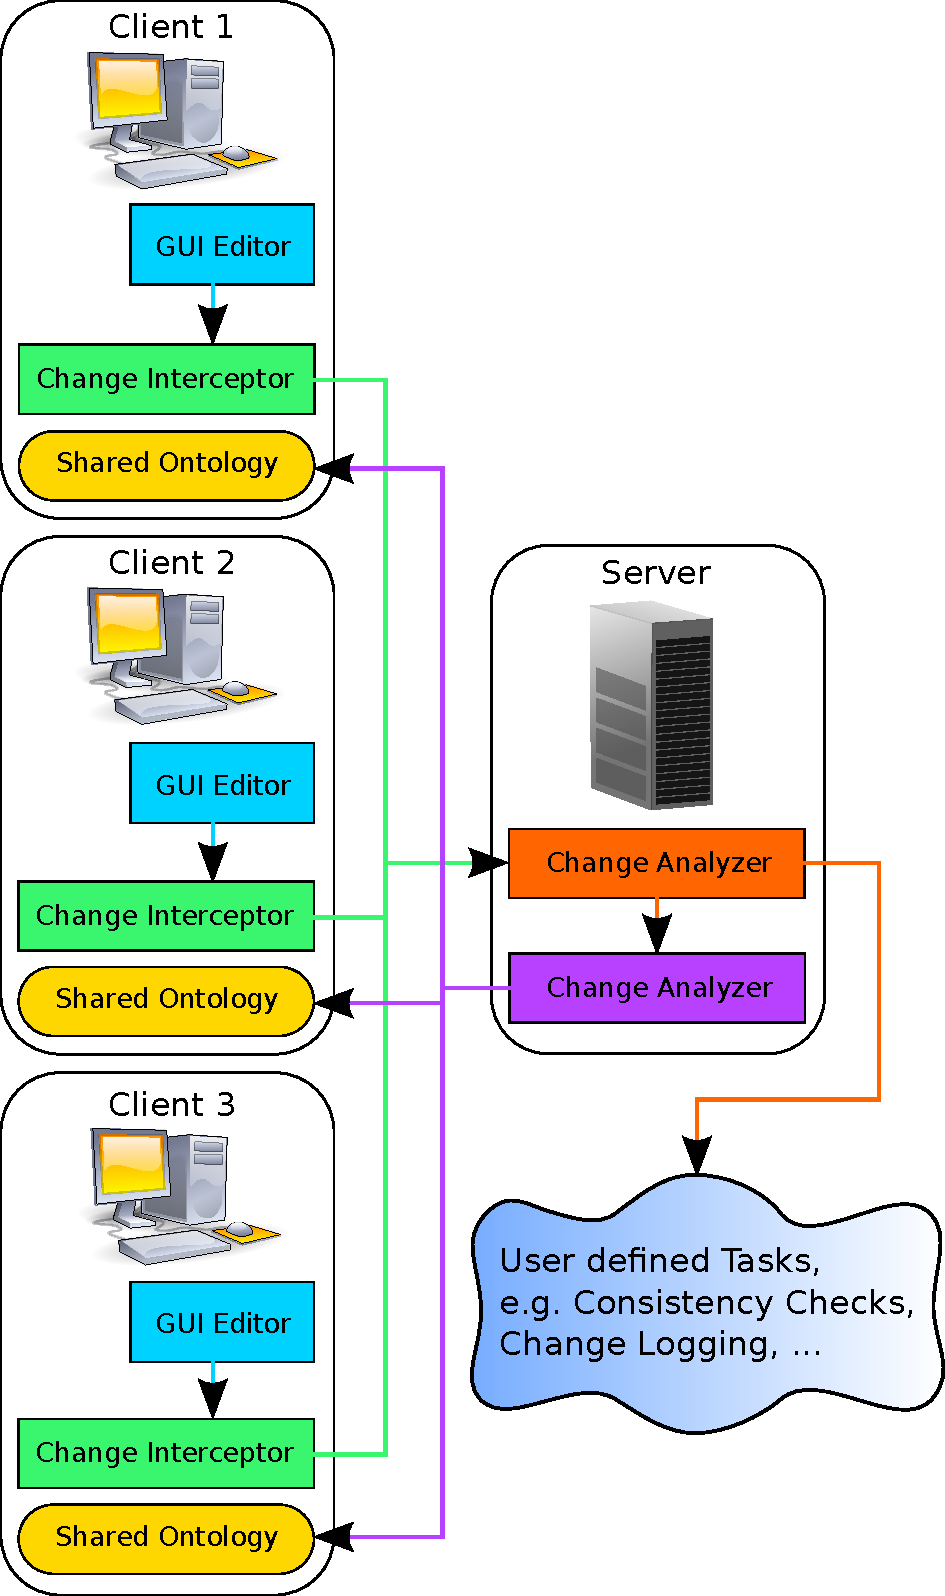
\includegraphics{BilderFrameworkArch/scenario0.pdf}
                                                }
                                        }
                                }
                                \label{img_scenario0}
                        }
                        \subfloat[Usage scenario 2]{
                                \rotatebox{0}{
                                        \resizebox{!}{0.6\textwidth}{
                                                \fbox{
                                                        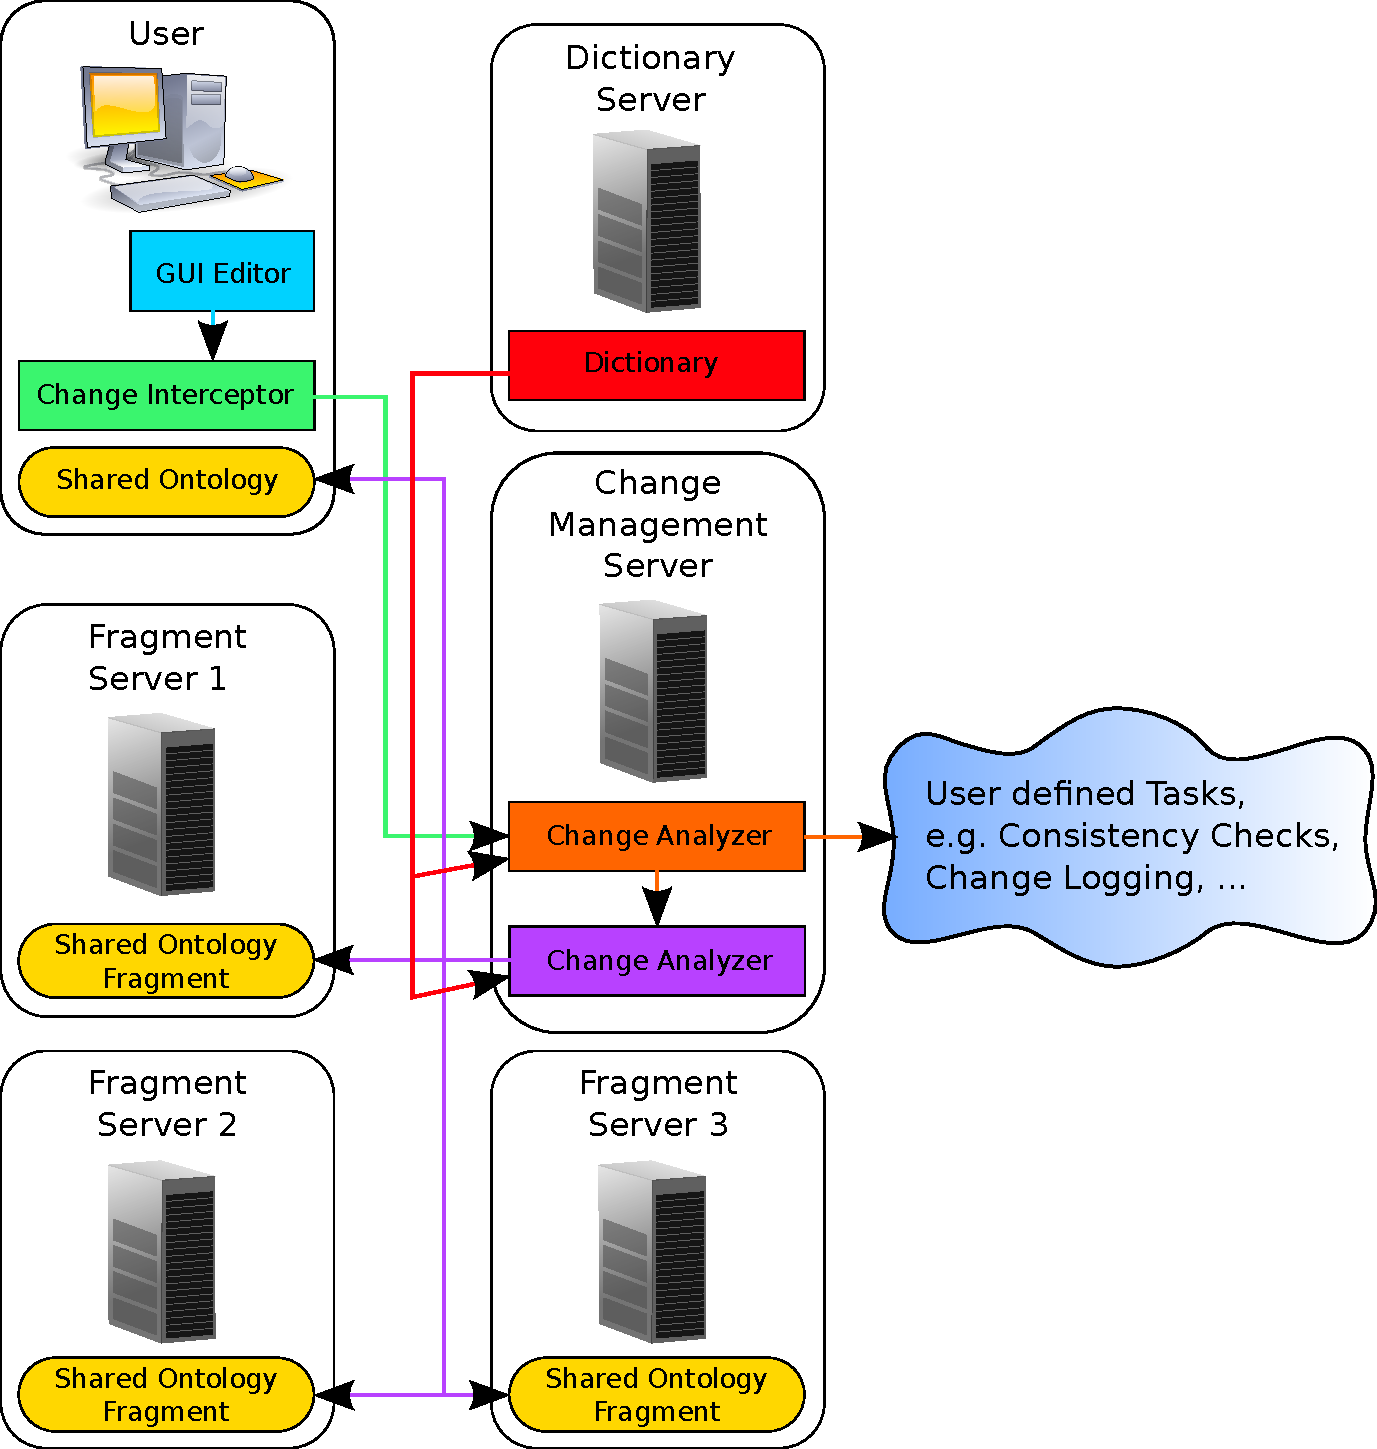
\includegraphics{BilderFrameworkArch/scenario1.pdf}
                                                }
                                        }
                                }
                                \label{img_scenario1}
                        }
        \label{fig_sharedontowizard}
\end{figure}
%\begin{figure}[h]
%       \caption{Usage scenario 1}
%       \begin{center}
%               \rotatebox{-90}{
%                       \resizebox{!}{0.45\textwidth}{
%                               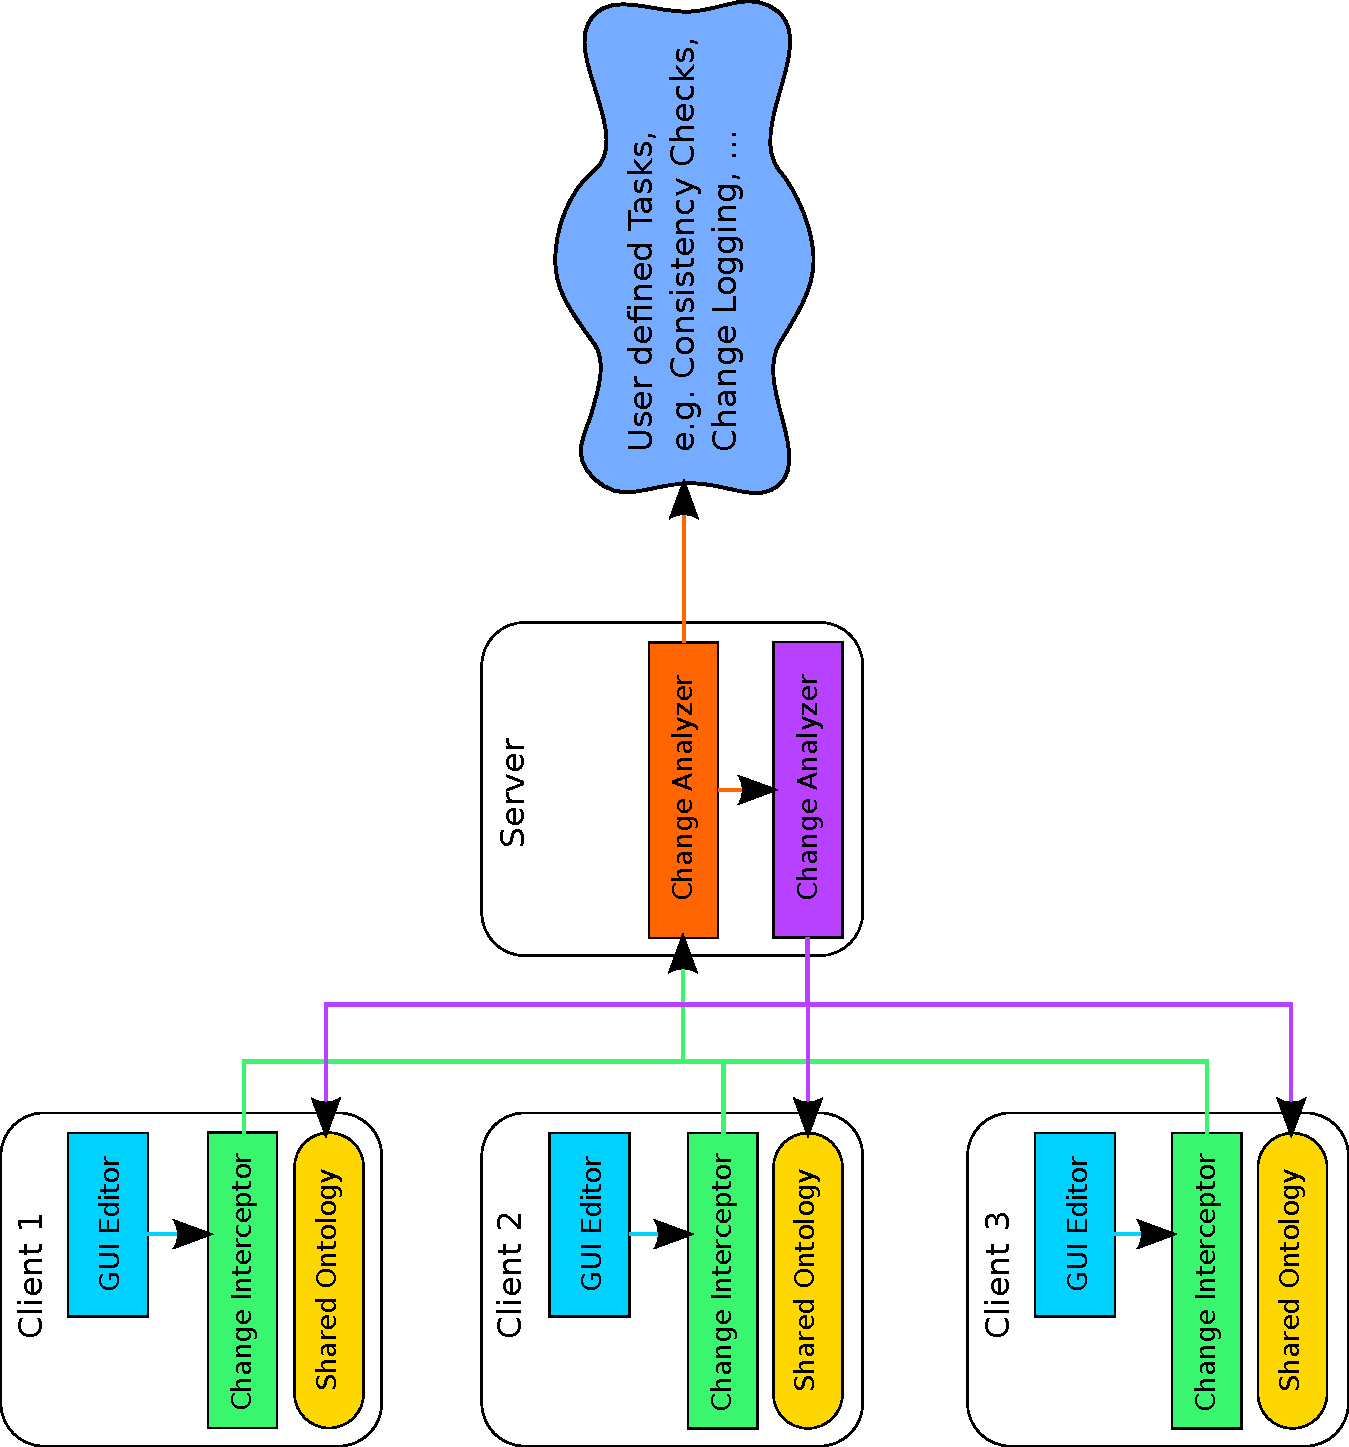
\includegraphics[width=10cm]{BilderFrameworkArch/component_overview0.pdf}
%                       }
%               }
%       \end{center}
%       \label{img_changemanagement}
%\end{figure}
%\begin{figure}[h]
%       \caption{Usage scenario 2}
%       \begin{center}
%               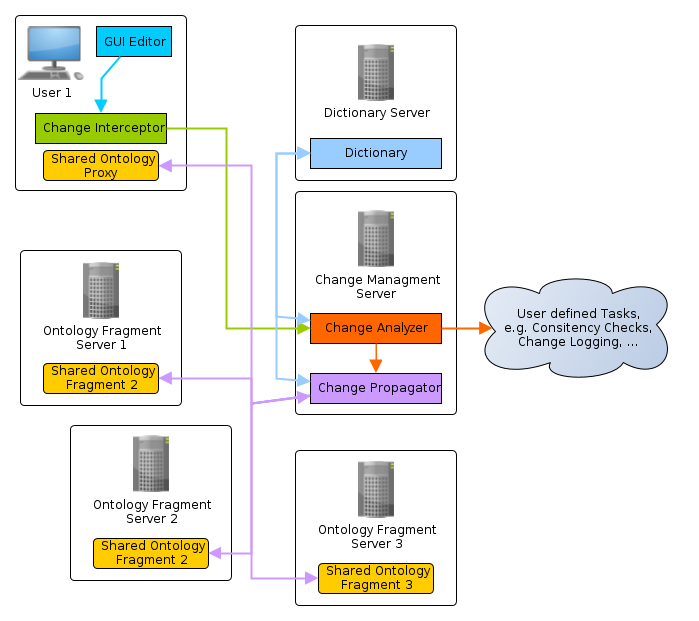
\includegraphics[width=10cm]{BilderFrameworkArch/component_overview2.png}
%       \end{center}
%       \label{img_changemanagement2}
%\end{figure}

\subsection{Shared Ontology}
\label{sharedOntology}
The key concept of the framework is the concept of a \emph{shared ontology}.
A shared ontology is an ontology which can be accessed and modified by
multiple clients. Working on a shared ontology is done synchronously which
means that changes are visible to all clients immediately after they have been made.
The defintion of a \emph{shared ontology} is based on the definition
in \cite{diaz2006}.

\begin{definition}[Shared Ontology] If an ontology is developed
through by publishing ontological contribution in contrast to developing
it through externalization we call it a \emph{Shared Ontology}.
\end{definition}

A shared ontology may be fragmented in smaller pieces which together
form the whole ontology. So a fragment is a subset of statements of the
ontology and is therefore an ontology itself.
Fragments can either be modular or non-modular.
Using modular fragments exposes several advantages which has been described
before in section \ref{modularization}.

\begin{definition}[Shared Ontology Fragment]
\label{sharedOntologyFragment}
For a Shared Ontology $o$ a set of axioms $\varphi$ is called a \emph{Shared Ontology Fragment}
of $o$ when $\varphi\subseteq o$.
\end{definition}

\subsection{Dictionary}
\label{dictionary}
The global dictionary contains meta information about fragments.
It covers fragment identifiers as well as fragment ontology signatures
and the \emph{identifier function} to look up a fragment by signature
and vice versa and is part of a distributed ontology system as proposed
in \cite{chen09}.
\begin{definition}[Identifier Function]
For a set $\mathcal{I}$ of ontology identifiers
and a set $\mathcal{F}$ of Shared Ontology Fragments
a bijective function $\phi$ : $\mathcal{I} \to \mathcal{F}$ that unambiguously assigns an identifier to every fragment is called an \emph{identifier function}.

\end{definition}
\begin{definition}[FragmentID]
For a set $\mathcal{I}$ of ontology identifiers,  a set $\mathcal{F}$ of Shared Ontology Fragments and a fragment $\varphi \in \mathcal{F}$, an identifier $\iota$ is called a \emph{FragmentID} of $\varphi$ if an identifier function $\phi$ exists such that $\exists \iota \in \mathcal{I} : \phi(\iota) = \varphi$. 
\end{definition}
Each Shared Ontology Fragment has a unique ID.
\begin{definition}[Dictionary]

For a set of FragmentIDs $\mathcal{I}_\varphi$, a set of Shared Ontology Fragments $\mathcal{F}$ and signature $\Sigma = \{{\sigma(\varphi)}\mid\varphi\in{\cal F}\}
$,
and $\phi$ an identifier function from ${\cal I}_\varphi$ to $\cal F$,
a triplet $\mathcal{D} = \{\mathcal{I}_\varphi, \Sigma, \phi \}$ is called
\emph{Dictionary}.

%\begin{enumerate}
%   \item $\Upsilon = \{ \iota set of fragment IDs
%   \item A set of ontology signatures $\Sigma = \bigcup_{i=1...n}{\sigma_i}$
%   \item Two functions $\phi$
%      $\texttt{getSignature} : \texttt{FragmentID} \to \texttt{Signature}$\\
%      $\texttt{getFragment} : \texttt{Signature} \to \texttt{FragmentID}$
%\end{enumerate}
\end{definition}
This offers the possibility to look up which fragment holds required information
when performing a query against a distributed ontology which is also
the primary purpose of the dictionary.
The dictionary can be further extended to contain other information about fragments
if needed such as the fragment size or structural properties.

%\begin{enumerate}
%\item Each concept name $\DLConVar{A}\in N_C$ is an \ALC-concept description.
%\item The most general concept $\top$ and the unsatisfiable concept $\bot$ are \ALC-concept descriptions.
%\item If \DLConVar C, \DLConVar D are \ALC-concept descriptions, and $\DLRolVar{R}\in N_R$, then  the concept conjuntion $\DLConVar C \DLand \DLConVar D$, the concept disjunction $\DLConVar C \DLor \DLConVar D$ and the concpet negation $\neg\DLConVar{C}$ are also \ALC-concept descriptions.
%\end{enumerate}


\newpage


\subsection{Distributed Ontology System}
\index{DOS}
We adapt the concept of a  \emph{Distributed Ontology System} (DOS)
proposed by \cite{chen09}. A DOS consists of a large shared ontology
a set of ontology fragments the ontology is composed of and a dictionary
to look up fragments.

\begin{definition}[Distributed Ontology System] For a large shared ontology
$o$, a set of ontology fragments $\mathcal{F}$ which $o$ is composed of
and a dictionary $\mathcal{D}$, a triplet $\{o,\mathcal{F},\mathcal{D}\}$
is called \emph{Distributed Ontology System}.
\end{definition}

\subsection{Change Management}
\label{changemanagement}
This sub section presents components related to change management in
the Replica Framework.

When it comes to the distribution of a shared ontology the Replica Framework has
to provide the means for managing changes. Each node provides special
components which allocate all necessary functionalities for \emph{change management}
from intercepting changes to analyzing and propagating them which are
also the three stages in order in which change is processed.

\subsubsection{Change Model}
The framework does not force the user into using a certain change distribution
model. By exhausting the full functionality of the change management
the Replica Framework offers the flexibility to implement change management
according to user's demands.

The forms of ontology modifications are diverse. Users can add or
remove axioms to shared ontologies or certain fragments, add annotations
or change the ontology ID. Moreover users may want to apply a set of these
modifications. Keeping track of modifications is essential in many applications
for example in versioning systems.

\begin{definition}[Change]
For the set $\Delta$ of ontology modifications, user ID $\upsilon$,
time~stamp~$\tau$, comment $\omega$, the 4-tuple 
$\mathcal{\nu} = \{\Delta, \upsilon, \tau, \omega \}$ is called \emph{change}.
\end{definition}
The Replica Framework uses a special container called \emph{change} to
carry a set of modifications, a user ID, a timestamp and a comment which
is meant to report the cause of the change.
%\begin{tabular}{ l l }
%Change: applyChange(c)

\begin{definition}[Criterion] 
A \emph{criterion} is a function $Change \to Boolean$ that
 \emph{matches} a change.

\end{definition}
Note that a \emph{Change} can contain a set of modifications.

\begin{definition}[Change Filter]
For $n \in \mathbb{N}$, Criteria $\gamma_i$, 
$\Theta = \bigcup_{i=0..n} \gamma_i$ is called \emph{Change Filter}.
\end{definition}
A \emph{Change Filter} is meant to be used at the first step of the change
processing but also in any other component where changes are handled.

\subsubsection{Change Processing}
Change processing in the Replica Framework follows a scheme which can be
modified if needed. Developers can implement custom modifications and
other tasks in any component. Figure \ref{img_changeprocessing} presents
the change processing work flow.
\begin{figure}[h]
        \caption{Change processing work flow}
        \begin{center}
                 \rotatebox{-90}{
                        \resizebox{!}{10cm}{
                                
\includegraphics[width=10cm]{BilderFrameworkArch/change_processing_flow.pdf}
                        }
                }
        \end{center}
        \label{img_changeprocessing}
\end{figure}\\
Whenever a change is applied this procedure is triggered. Next change
processing is described in algorithm \ref{alg_applychange} which
describes the change processing in detail.
\begin{algorithm}[h]                      % enter the algorithm environment
\caption{\textsc{ApplyChange($\mathcal{\nu}$)}}          % give the algorithm a caption
\label{alg_applychange}                           % and a label for \ref{} commands later in the document
\begin{algorithmic}[h]                    % enter the algorithmic environment
\REQUIRE Shared Ontology $o$, Change Filter $\Theta$
\IF{\NOT \textsc{Filter($\mathcal{\nu}, \Theta$)}}
        \STATE{$\alpha \leftarrow \textsc{Analyse($\mathcal{\nu}$)}$
        \STATE \textsc{Trigger($\alpha$)}
        \STATE \textsc{Propagate($\alpha,\mathcal{\nu}$)}}
        \RETURN applied changes on $o$
\ELSE
        \STATE // ignore change
\ENDIF
\end{algorithmic}
\end{algorithm}\\
The other procedures used in algorithm \ref{alg_applychange} are:
\begin{algorithm}[h]                      % enter the algorithm environment
\caption{\textsc{Filter($\mathcal{\nu}, \Theta$)}}          % give the algorithm a caption
\label{alg_filter}                           % and a label for \ref{} commands later in the document
\begin{algorithmic}[h]                    % enter the algorithmic environment
\REQUIRE Criteria $\chi_i \in \Theta$\hspace{0,5cm} $i = 1,2,...,n$\hspace{0,5cm} $i,n \in \mathbb{N}$
\FOR{$i = 1\text{ to }n$}
        \IF{$\chi_i(\mathcal{\nu})$}
                \RETURN \TRUE
        \ENDIF
\ENDFOR
\RETURN \FALSE
\end{algorithmic}
\end{algorithm}
\begin{itemize}
        \item[\textsc{Analyse}]  is a developer-defined analysis procedure that examines a change
        and returns an analysis as a result. The Replica Framework poses no
        restrictions on the subject and content of this analysis.
        \item[\textsc{Trigger}] is also a developer-defined algorithm that depends on the
        analysis. This algorithm may for example be a consistency check of
        the ontology or protocolling a change.
        \item[\textsc{Propagate}] is the function that sends a change to other peers.
        To which peers the change is sent depends on the developers demands.
        The change can also be modified at this stage.
\end{itemize}

%\begin{algorithm}[h]                      % enter the algorithm environment
%\caption{\textsc{Analyse($\mathcal{\nu}$)}}          % give the algorithm a caption
%\label{alg_analyses}                           % and a label for \ref{} commands later in the document
%\begin{algorithmic}[h]                    % enter the algorithmic environment
%\REQUIRE Shared Ontology $\mathcal{O}$
%\STATE $\alpha \leftarrow$ Create change analysis
%\STATE \textsc{Trigger($\alpha$)}
%\RETURN $\alpha$
%\end{algorithmic}
%\end{algorithm}

\subsubsection{Change Interceptor}
The \emph{Change Interceptor} is responsible for intercepting and if required
filtering changes on the shared ontology. Filters are be based on the node
a change originates from and also the kind of change.

This component is local on a node. After a change has been intercepted
it is either modified and forwarded to the change analyzer or filtered.

\subsubsection{Change Analyzer}
The \emph{Change Analyzer} component is used to inspect the change type
and possibly trigger user defined tasks connected to certain outcomes of the
analysis. A user defined task may for example be a consistency check or some
other kind of check for constraints. This offers workflow support.

Changes can also be filtered at this component. The main difference to the
change interceptor is that the change analyzer can either be distributed thus 
local on any node or at certain user specified hosts. This allows centralizing
change analysis and easy change tracking for building change histories.

\subsubsection{Change Propagator}
\label{changepropagator}
At last the \emph{Change Propagator} component is required to send the
shared ontology change to all or some other nodes. The Change Propagator
should know the analysis of the change produced by the Change Analyzer.
In addition to that a change propagation strategy should be configurable. The
strategy determines which changes will be sent to specified nodes.
It is therefore a very important aspect of the framework. The strategy can either
be configured to propagate changes to all or just some nodes.
The target node(s) of a certain change can also depend on the kind of change
which is about to be propagated or other developer defined information.


\subsection{Communication Node}
The framework relies on a client and server communication model.
Clients connect to a server and can then retrieve shared ontologies managed
by the server they are connected to as well as changes and communication
data from other clients. As centralization is not always desired the
framework also allows for building decentralized network structures
by employing the concept of a \emph{communication node}.
A communication node is a peer that provides client as well as server functionality.

The concept of a communication node is similar but not equal to the
peer concept of a peer-to-peer network. Table \ref{p2pRepComparison}
offers a comparison between the two ideas which is based on the definition
of a peer-to-peer network by \cite{schollmeier01}.
The major difference between both network models is that in opposite to
a self-organizing peer-to-peer network communication node management has
to be configured manually.

\begin{table}[h]
        \centering
        \caption{Comparison of peer-to-peer and Replica Framework peer concepts}
        \label{p2pRepComparison}
        \begin{tabular}{ | p{0.60\textwidth} | c | c | }
                \hline
                \textbf{Characteristic} & \textbf{Peer-to-Peer} & \textbf{Replica Framework} \\ \hline
                Heterogenity of network connection speed, performance, reliability & yes &  yes \\ \hline
                Peers provide services and resources and request services of other peers & yes & yes \\ \hline
                Services and resources can be shared across all peers & yes & yes \\ \hline
                Peers make up an overlay network & yes & yes \\ \hline
                Peers are autonomous & yes & yes \\ \hline
                The network is self-organizing & yes & no \\ \hline
        \end{tabular}
\end{table}

\section{Behavioral Aspects}
This section outlines an important behavioral aspect of the Replica Framework
architecture. \emph{Change Management} is described, the
concept and a simple standard management strategy that a
framework implementation should provide as a starting point.

\subsection{Change Management}
\label{changemanagement_behave}
In some usage scenarios not all users may be allowed to submit changes or
enforcing restrictions is necessary. Furthermore changes may need to
be modified before applying them to the shared ontology or it may be necessary
to trigger an event when a certain type of change is submitted.
Performing a consistency check before applying a change is an example for
such a situation where change management is required.

To offer a maximum of flexibility a change can be filtered and modified
at any stage in change processing: (1) interception (2) analysis (3) tasks
and (4) propagation.

\subsubsection{Change distribution}
A fundamental aspect of change management is the distribution of changes.
The easiest change distribution model is plain synchronous unmodified change
distribution. All changes made on a node are instantly transmitted without
modification. By defining a change propagation strategy for the
\emph{change propagator} component presented in section \ref{changepropagator}.


\section{System Configuration}
Each Replica Framework component may require a configuration supplied by the user.
Whenever possible reasonable defaults are used which can then be overridden by
supplied configuration values. To simplify the configuration process a bundle
of the individual component configurations can be created and be read at
a central place. The Replica Framework takes care of distributing and applying
the configurations to corresponding components.


\chapter{Implementation of the Backend}
\label{backendimplementation}
\index{Object-oriented programming}
\index{Aspect-oriented programming}
\index{OWLAPI}
To implement the backend side of the framework a combination of object-oriented
programming (OOP) and aspect-oriented programming (AOP) was chosen.
AOP was applied with the
intention to improve the development of the change interception mechanism of the shared
ontology described in \ref{sharedOntologyImpl} and security related concerns as AOP
is suited well for implementing cross-cutting concerns.

To support the development procedure unit tests for all modules were implemented to
ensure components remain functional in the course of the development.

The code convention was adapted to the OWLAPI's to ease entry for beginners that
are familiar with the OWLAPI.


%%%%%%%%%%%%%%%%%%%%%%%%
\section{Technologies}
This section describes the technologies used in this project, reasons
why they have been chosen and experiences in the course of the development.

\subsection{AspectJ}
\index{AspectJ}
\index{Aspect-oriented programming}
AspectJ\footnote{AspectJ \url{http://eclipse.org/aspectj/}} is an open-source
project of the eclipse foundation and extends Java with AOP.
AspectJ is great for implementing tracing logging or
other security related concerns.

In the context of the Replica Framework it was meant to implement 
change interception at first. During the course of the project the 
AspectJ change interception mechanism was replaced with native Java 
code for practical reasons. Although AspectJ is not thoroughly used anymore
in the project it is still included as it can be used to implement security
and logging issues if needed by the developer. The main interface of the
shared ontology is prepared to allow easy creation of aspects in 
regard to shared object access. All shared object methods have a 
special annotation defined by the marker interface \emph{ProxyMethod}.
Additionally methods which modify the shared ontology object carry the
\emph{PropagatingMethod} annotation as these methods require change
propagation as shown in listing \ref{applyChange}.

A major drawback of using AspectJ in this project was the impact on
performance and memory usage when implementing change interception and
propagation with AspectJ.

\subsection{Eclipse Communication Framework}
\index{ECF}
The Eclipse Communication Framework\footnote{Eclipse Communication 
Framework \url{http://www.eclipse.org/ecf/}} (ECF) is a mature framework for 
building distributed servers, applications and tools. In contrast to 
other communication frameworks does ECF not implement a single 
communication protocol but relies on protocol independence instead. It 
is therefore an abstraction of many well known communication 
techniques and protocols. This framework implements a sophisticated 
extendable model which hides underlying protocols with unifying APIs 
for communication functionalities. These include currently APIs for
file transfer, implementing remote services, presence, service 
discovery, messaging and object replication. ECF is actively developed,
has a lot of components and features, along with the fact that the protocol
independence and extendability principle offers a lot of flexibility 
this was the communication framework of choice for this project.

A single but important shortcoming of ECF is the fragmented and 
incomplete documentation. For many components there is neither an official
nor an unofficial documentation available which had a significant 
impact on the progress of the project development.

%%%%%%%%%%%%%%%%%%%%%%%%
\section{Modules}
\index{OSGi}
Modules represent a separation of concerns by packing functionality in logical units. Modular
Programming therefore allows to build large and complex applications while improving
maintainability.

The framework components are organized in modules which are implemented
as OSGi\footnote{The OSGi Alliance is a worldwide consortium of technology innovators that
advances a proven and mature process to create open specifications that enable
the modular assembly of software built with Java technology.} Bundles.
Bundles are a collection of Java source files together with libraries and meta information.
A special file \emph{MANIFEST.MF} holds meta information such as bundle name and version,
vendor name, required execution environment, exported packages and dependencies.

Dependency management is a very important feature of the OSGi framework.
This section offers an overview of all Replica Framework modules and
describes the \emph{Core} and \emph{Communication} modules in detail. These modules are
entry points to the Replica Framework.

\subsection{Core module}
The core module is the one on which all other modules depend on.
It contains an implementation of the Shared Ontology described in section \ref{sharedOntology}
and the class \emph{OWLReplicaManager} which is the entry point to the framework.
\emph{OWLReplicaManager} has the same functionality as the \emph{OWLManager}
in the \index{OWLAPI}OWLAPI.

Moreover the core module contains a builder which generates an abstract shared ontology
implementation. This builder can be used from the command line and was made
for the purpose of reducing maintenance costs in case the OWLAPI is updated.

\subsection{Communication module}
\label{communicationmodule}
The communication module contains all communication-related components of
the framework. The \emph{CommManager} can be used to create connection instances
and is required on both the client and server side.

In addition to that does the communication module include the \emph{channel} package.
This package contains an implementation of the \emph{SignalChannel} which is a slight
addition to the ECF \emph{Datashare API} message concept. \emph{SignalChannel} is meant
to be used in application development when communication requires transmission
of events or other relatively small typed messages.


\newpage


\subsection{Overview}
This sub section offers an overview of all Replica Framework modules in
table \ref{frameworkplugins}.
\begin{table}[h]\centering
	\caption{Overview of all Replica Framework plugins}
	\label{frameworkplugins}
	\begin{tabular}{ | c | p{9cm} | c | }
		\hline
			\begin{tabular}{ c }
				\textbf{\emph{Bundle Postfix}},\\
				\textbf{Module Name}
			\end{tabular} & \textbf{Description} & \textbf{Dependencies} \\ \hline
		\begin{tabular}{ c }
			\emph{owlapi}
		\end{tabular} & The OWLAPI lib Plug-in plugin contains the patched version of
			the OWLAPI library. & - \\ \hline
		\begin{tabular}{ c }
			\emph{core}
		\end{tabular} & The core plugin contains the Shared Ontology Implementation and Shared Ontology
			builder which is required when applying OWLAPI updates. &  \emph{owlapi} \\ \hline		
		\begin{tabular}{ c }
			\emph{app}
		\end{tabular} & The application plugin contains interfaces and classes required
			to build applications like server or client instances. & \emph{core} \\ \hline
		\begin{tabular}{ c }
			\emph{comm}
		\end{tabular} & The communication module contains all communication related components
			of the Replica Framework. Especially the
			\emph{CommManager} is included in this plugin. & \emph{core} \\ \hline
		\begin{tabular}{ c }
			\emph{dictionary}
		\end{tabular} & The dictionary plugin plugin holds interfaces and classes
			related to the Dictionary concept of the Replica Framework. & \emph{core} \\ \hline
		\begin{tabular}{ c }
			\emph{fragments}
		\end{tabular} & The fragments plugin bundle incorporates the Shared Ontology
			Fragment concept related components of the Replica Framework. & \emph{core} \\ \hline
		\begin{tabular}{ c }
			\emph{changes}
		\end{tabular} & The Change Management plugin
			holds special implementations of the \emph{OWLReplicaOntology}
			interface that actualize all necessary parts of the
			Change Management concept of the framework. & \emph{core}, \emph{fragments} \\ \hline
		\begin{tabular}{ c }
			\emph{neonplugin}
		\end{tabular} & The NeOn Toolkit plugin includes the implementation of the
			NeOn Toolkit plugin. & \emph{core}, \emph{comm} \\ \hline
		\begin{tabular}{ c }
			\emph{plicies}
		\end{tabular} & This plugin
			contains components required for \emph{policy management}.
			It has not yet been implemented at the time of writing.
			& \emph{core} \\ \hline
		\begin{tabular}{ c }
			\emph{query}
		\end{tabular} & This plugin holds Query Management related
			parts. It has not yet been implemented at the time of writing. & \emph{core} \\ \hline
		\begin{tabular}{ c }
			\emph{demo}
		\end{tabular} & This plugin contains an implementation of a
			standalone demonstrator application that presents features of
			the Replica Framework. & \emph{core}, \emph{comm} \\ \hline
	\end{tabular}
\end{table}


\newpage


\section{Shared Ontology Implementation}
\label{sharedOntologyImpl}
The shared ontology object is a fundamental component of the framework.
The \emph{OWLReplicaOntology} interface is a facade combining the 
OWLAPI \emph{OWLOntology} interface with the ECF \emph{ISharedObject} interface.
To provide implementations of this interface was a challenging task.
As Java supports multiple inheritance only for interfaces it is impossible
to extend from existing implementations of both respective interfaces.
Consequently implementations can only extend from either the 
\emph{OWLOntology} or \emph{ISharedObject} implementations exclusively.
The problem is that the effort of implementing all methods of both interfaces and
maintaining these over time with updates of both the OWLAPI and ECF
is way too high.

The solution is to create an implementation that extends 
\emph{TransactionSharedObject} a reference implementation of the ECF
ISharedObject interface in combination with the proxy pattern.
As the implementation has to provide all \emph{OWLOntology} methods as well it
contains an ontology as an attribute. The method calls are then
delegated to this inner ontology object.
To simplify the process of creating such a class in case of an OWLAPI update
the framework provides a builder for an abstract class with the structure
described before.

\subsection{Change Interception}
Intercepting changes on the ontology instance is essential for the
implementation of a shared ontology and change management in the
context of distributed ontology system. At first AspectJ was used to
leverage the strength of crosscutting-concerns in AOP. The idea was
to intercept changes by declaring pointcuts containing all join points
that denote ontology changes. Filtering, modification and propagation
was implemented in corresponding advices then.

When implementing change management the complexity of the AOP approach
became unbearable. Aside from that crosscutting-concerns broke with
the principle of separation of concerns fundamental to modular programming.
Mixing both approaches was therefore problematic and impractical so
falling back to a traditional object-oriented programming solution was
the proper alternative. The solution was to intercept changes in the 
outer ontology proxy methods responsible for applying changes
before passing them to the inner ontology object as shown in listing
\ref{applyChange}. To avoid cycles when propagating changes, another
method is required which bypasses change processing and a distinction
between callers as shown in listing \ref{applyChangesSilent}.

This approach brought a slight performance improvement
as the AspectJ runtime was not required anymore and the amount
of method invocations was reduced.

%%%%%%%%%%%%%%%%%%%%%%%%
\section{Communication}
To implement a useful collaborative ontology development system it is not
enough to provide only a shared ontology. The framework should also provide
the means to build other components that support in the process of collaborative
ontology development.

Furthermore communication should be reliable and ideally fault-tolerant. This
was accomplished by transactional message propagation. ECF provides a
special \emph{ISharedObject} implementation called \emph{TransactionSharedObject}
for all-or-nothing, in-order messaging. Using this feature ensures that changes
are either applied correctly or dropped. No partial changes can be applied
which greatly reduces the risk of raising inconsistencies in case of communication
errors.

\subsection{Connection Management}
The main component which is used for connection management is the \emph{communication manager}.
It can be used to create multiple connections. A connection provides access
to the basic communication facilities. These include the ECF interfaces
for managing shared objects and messaging as well as the \emph{signal channel manager}.

\subsubsection{Connection Activity}
To avoid blocking methods when communicating asynchronously a mechanism
is needed which allows sending messages and reacting to a response
or a timeout later without waiting for the result.
A \emph{connection activity} represents a procedure in the context of a connection.

It contains a list of states and user-defined transitions between these
states.
%This is best explained with a simple example. Consider a client wants
%to add a new shared ontology.
%Therefore in terms of the communication two messages are necessary:
%(1) the client sends a request for a new shared object ID
%(2) the server responds the new ID.\\
%When the client sends the request \todo[inline]{code}

\subsection{Signals}
In some situations messaging may be restricted to sending simple typed
messages that trigger certain predefined tasks. For example refreshing
the screen or rebuilding an repository index. For this purpose \emph{Signals}
have been introduced which are asynchronous messaging based and allow
for sending plain typed messages without content or typed messages with
content.



%%%%%%%%%%%%%%%%%%%%%%%%
\section{Change Management}
\index{AspectJ}
Change management implementations are hidden behind the \emph{OWLReplicaOntology}
interface. The principle is that changes are intercepted before submitting
them to the Ontology object within the OWLReplicaOntology object and
processing them. The various components of that processing chain are
described in section \ref{changemanagement}.
At first AspectJ was used to realize ontology change interception.
A special marker interface called \emph{PropagatingMethod} indicates
which methods in the \emph{OWLReplicaOntology} have a modifying impact
and are therefore part of the change management.


%%%%%%%%%%%%%%%%%%%%%%%%
\newpage
\section{Applications}
The Replica Framework comes with three applications that make it possible
to use the framework.
This section describes the communication hosts briefly that
the Replica Framework includes.
These are the \emph{server}, \emph{client} and \emph{node} hosts.

\subsection{Server}
The \emph{server} application of the Replica Framework is a central spot for
clients to connect to and to hold meta information of all clients and
shared ontologies. That is why the server can also be seen as some kind
of \emph{shared ontology repository}.

Servers also manage the shared ontologies. For example when clients create a shared
ontology they need to retrieve a shared ontology ID from the server before.
Whenever a client needs to access a shared ontology it has to connect to
a server.

\subsection{Client}
The \emph{client} application of the Replica Framework can retrieve lists of
shared ontology IDs from the server. It is used to communicate with the
server for accessing shared ontologies.

In addition to that it allows to retrieve and add \emph{shared ontology groups}
which are meant to simplify the implementation of shared ontology management.
Such a group consists of a set of shared ontologies.
A shared ontology can also occur in more than one group.

\subsection{Node}
A \emph{node} is a special host that combines the functionality of
servers and clients. Its primary purpose is to ease the development of
peer-to-peer applications in the context of Distributed Ontology Systems.
The implementation is basically an instance of a server and a client
hidden behind the \emph{ReplicaOntologyNode} interface.


\subsection{System Configuration}
To configure the Replica Framework a configuration has to be specified.
This configuration consists of sections for each component. Wherever
possible reasable defaults are used so that the supplied configuration
overwrites configuration values. This principle is meant to ease system
configuration.

Support of runtime changes of configuration values is preferred wherever
possible. For example the configuration for the creation of connections
with the \emph{CommManager} of the communication module described in section
\ref{communicationmodule} can be changed after the \emph{CommManager}
has been started. This configuration sets defaults for
new connections but specific parts of it or the whole configuration of
a connection can also be supplied to the \emph{CommManager} when a connection
is about to be created.


%\begin{table}[H]
%\centering
%\footnotesize % alternativ \tiny \scriptsize \footnotesize \normalsize \large ...
%\begin{tabular}{|c|c|c|c|c|}\hline
%\bf Filename & \bf Originating project & \bf Used in bundles & \bf License & \bf Description	\\ \hline
%org.aspectj.runtime.jar  &  AspjectJ &  all &  EPL 1.0  &  AspectJ runtime	environment 	\\ \hline
%org.aspectj.weaver.jar  &  AspjectJ &  all &  EPL 1.0  &  AspectJ weaver 	\\ \hline
%ajde.jar  &  AspjectJ &  all &  EPL 1.0  &  AspectJ weaver 	\\ \hline
%\end{tabular}
%\caption{Table of libraries used}
%\label{hd44780befehle}
%\end{table}

\chapter{Implementation of Demonstrations}\label{chp-demonstrations}



\section{NeOn Toolkit Plugin Implementation}
This section describes the NeOn Toolkit the Replica Framework NeOn Toolkit
plugin implementation and presents screenshots of the plugin.

\subsection{NeOn Toolkit Platform}
\index{NeOn Toolkit}
\begin{wrapfigure}{r}{0.5\textwidth}
        \caption{NeOn Toolkit editor GUI}
        \begin{center}
                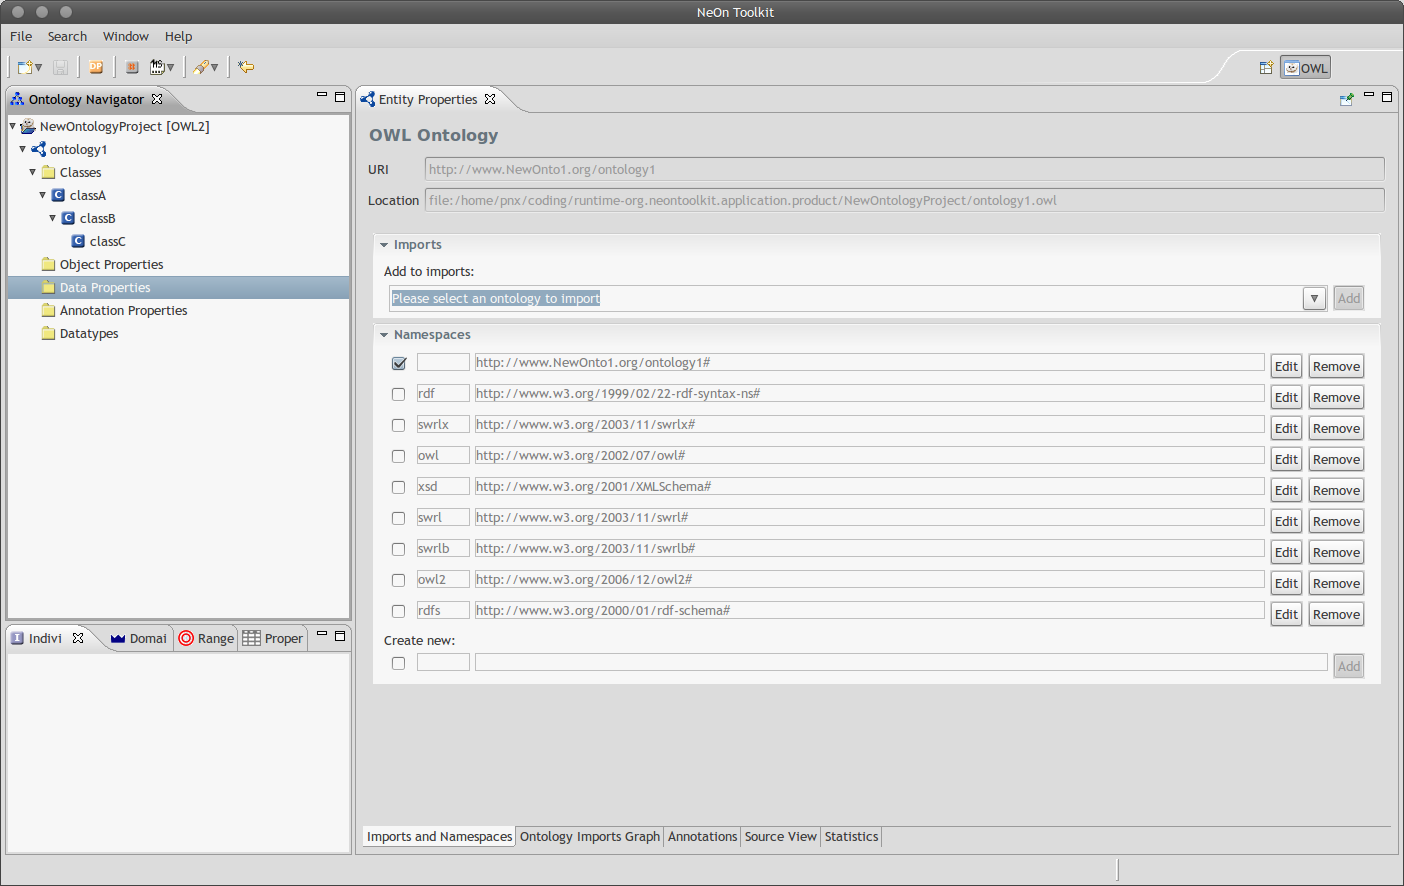
\includegraphics[width=0.5\textwidth]{BilderFrontendImpl/editor.png}
        \end{center}
        \label{fig_editor}
\end{wrapfigure}
The NeOn Toolkit is an ontology engeneering environment implemented as
a desktop application built on the code-base of \index{OntoStudio}
OntoStudio\footnote{OntoStudio is a commerical engineering environment of 
ontoprise, \url{http://www.ontoprise.de/}}, which is in turn based on the
popular IDE Eclipse\index{Eclipse}. The application is implemented as an
Eclipse application with the advantage that the application uses the proven
Eclipse application model and tools of the Eclipse platform.
Technically an Eclipse application is a special plugin which is started
by the eclipse platform. In contrast to usual plugins the lazy-loading
principle does not apply to it and menus and toolbars can be customized
programmatically.

Apart from basic ontology creation the NeOn Toolkit features many other
ontology engineering tools that support in the ontology development lifecycle.

\subsection{Plugin Implementation}
\index{NeOn Toolkit}
The NeOn Toolkit is implemented as an \index{Eclipse}Eclipse\footnote{Eclipse a popular
free, open source \index{IDE}IDE \url{http://www.eclipse.org/}} application. Like
the IDE the application architecture relies on the \index{OSGi}OSGi module system and
service platform\footnote{The Eclipse development community therefore also provides an
implementation of the OSGi specification call Equinox \url{http://www.eclipse.org/equinox/}.}.
Thus the NeOn Toolkit plugin was implemented as an OSGi bundle containing
the necessary meta information required to integrate in the Eclipse
application system.

In addition to the main plugin the NeOn Toolkit bundle containing
the \index{OWLAPI}OWLAPI library had to be modified because the current Replica Framework
implementation requires a patched version.

The plugin integrates smoothly into \index{NeOn Toolkit}NeOn Toolkit and extends its functionality
by adding a Replica Framework project creation wizard and a wizard for
creating shared ontologies as shown in figure \ref{fig_sharedontowizard}.
%\begin{figure}[h]
%       \caption{Replica Framework project creation wizard}
%       \begin{center}
%               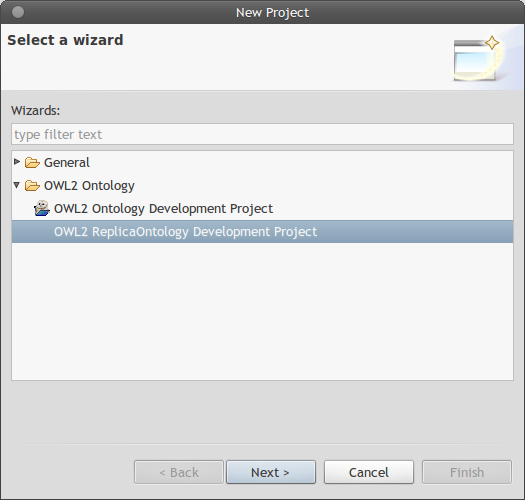
\includegraphics[width=\textwidth/2]{BilderFrontendImpl/wizard0.png}
%       \end{center}
%       \label{img_sharedontowizard0}
%\end{figure}\\
The shared ontology creation wizard also takes care of starting a local Replica Framework server and
initializing an empty shared ontology.

When a shared ontology has been created within a Replica Framework project
the NeOn Toolkit editor shown in figure \ref{fig_editor} can be used to modify
the ontology. All changes
of the ontology are then synchronized with all other connected editors which
enables simultaneous team based development.
\begin{figure}[h]
        \caption{Shared ontology creation wizard}
        \centering
                        \subfloat[Shared ontology project creation wizard.]{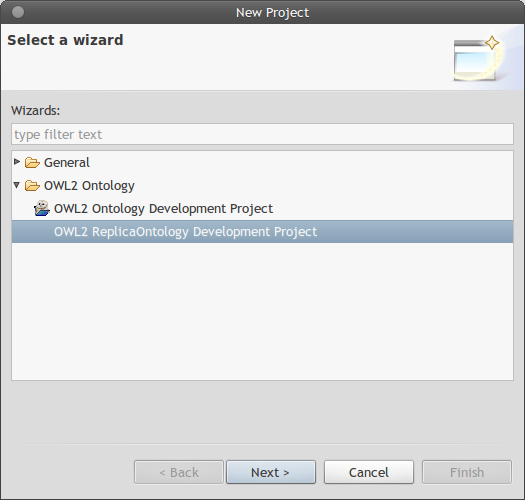
\includegraphics[width=0.45\textwidth]{BilderFrontendImpl/wizard0.png}}
                        \hspace{1cm}
                        \subfloat[Shared ontology project creation wizard.]{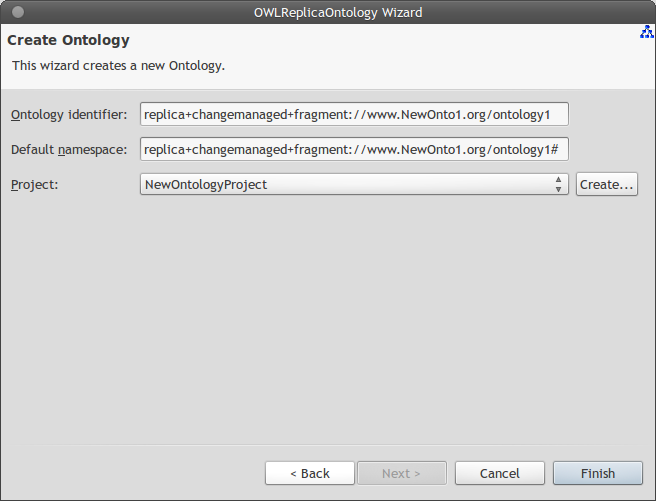
\includegraphics[width=0.45\textwidth]{BilderFrontendImpl/wizard1.png}}
        \label{fig_sharedontowizard}
\end{figure}


\newpage


\section{Replica Framework demonstrator}
\index{JUNG}
\label{replicademonstrator}
The Replica Framework demonstrator is a standalone application which uses the
JUNG\footnote{JUNG — the Java Universal Network/Graph Framework
\url{http://jung.sourceforge.net/}} network/graph framework to provide
an interactive demonstration of the framework's capabilities.

The demonstrator GUI has a graph view section, an information section
and a control section. Nodes in the graph correspond to \index{OWLAPI}OWLAPI classes.
Each client can add a sub node to any node in the graph. The color of
the node indicates the client the node originates from. Every window
functions as a client. When the demo starts up two clients connect to a
server instance.

Figure \ref{fig_demo} shows two demonstrator instances,
\textcolor{red}{\textbf{Client 0}} and \textcolor{green}{\textbf{Client 1}}
with a class hierarchy edited by both clients. The node colors indicate
the client the node originates from.
\begin{figure}[h]
        \caption{Replica Framework demonstrator}
        \begin{center}
                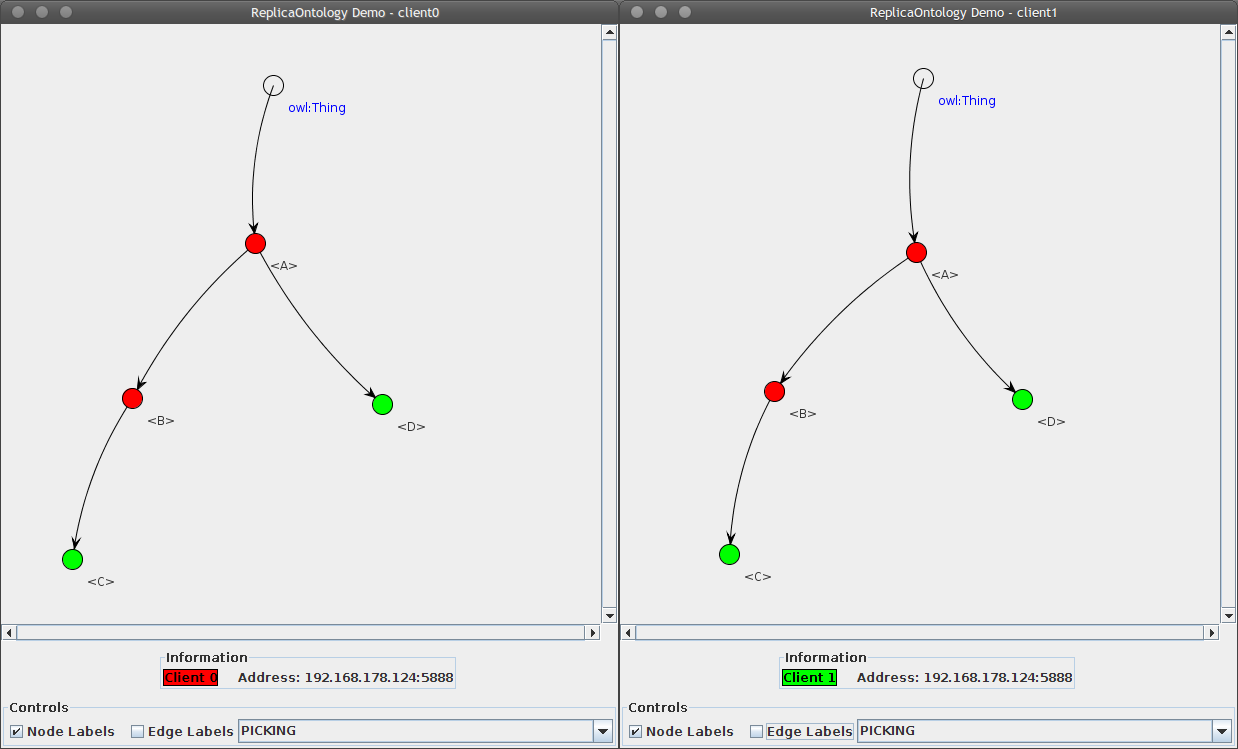
\includegraphics[width=\textwidth]{BilderFrontendImpl/demonstrator.png}
        \end{center}
        \label{fig_demo}
\end{figure}

%\begin{table}[H]
%\centering
%\footnotesize % alternativ \tiny \scriptsize \footnotesize \normalsize \large ...
%\begin{tabular}{|c|c|c|c|c|}\hline
%\bf Filename & \bf Originating project & \bf Used in bundles & \bf License & \bf Description       \\ \hline
%org.aspectj.runtime.jar  &  AspjectJ &  all &  EPL 1.0  &  AspectJ runtime     environment         \\ \hline
%org.aspectj.weaver.jar  &  AspjectJ &  all &  EPL 1.0  &  AspectJ weaver         \\ \hline
%ajde.jar  &  AspjectJ &  all &  EPL 1.0  &  AspectJ weaver     \\ \hline
%\end{tabular}
%\caption{Table of libraries used}
%\label{hd44780befehle}
%\end{table}





%\protect \addtocontents{toc}{\protect\newpage}  % Seitenumbruch im Inhaltsverzeichnis
%\cleardoublepage
%\chapter{Experimental evaluation}



\section{System parameters}
Lorem ipsum dolor sit amet, consectetur adipisici elit, sed eiusmod tempor incidunt ut labore et dolore magna aliqua. Ut enim ad minim veniam, quis nostrud exercitation ullamco laboris nisi ut aliquid ex ea commodi consequat. Quis aute iure reprehenderit in voluptate velit esse cillum dolore eu fugiat nulla pariatur. Excepteur sint obcaecat cupiditat non proident, sunt in culpa qui officia deserunt mollit anim id est laborum.

Duis autem vel eum iriure dolor in hendrerit in vulputate velit esse molestie consequat, vel illum dolore eu feugiat nulla facilisis at vero eros et accumsan et iusto odio dignissim qui blandit praesent luptatum zzril delenit augue duis dolore te feugait nulla facilisi. Lorem ipsum dolor sit amet, consectetuer adipiscing elit, sed diam nonummy nibh euismod tincidunt ut laoreet dolore magna aliquam erat volutpat.


\section{Ergebnisse zu Genauigkeit, Auf"-lösung und Wiederholrate}
Lorem ipsum dolor sit amet, consectetur adipisici elit, sed eiusmod tempor incidunt ut labore et dolore magna aliqua. Ut enim ad minim veniam, quis nostrud exercitation ullamco laboris nisi ut aliquid ex ea commodi consequat. Quis aute iure reprehenderit in voluptate velit esse cillum dolore eu fugiat nulla pariatur. Excepteur sint obcaecat cupiditat non proident, sunt in culpa qui officia deserunt mollit anim id est laborum.

Duis autem vel eum iriure dolor in hendrerit in vulputate velit esse molestie consequat, vel illum dolore eu feugiat nulla facilisis at vero eros et accumsan et iusto odio dignissim qui blandit praesent luptatum zzril delenit augue duis dolore te feugait nulla facilisi. Lorem ipsum dolor sit amet, consectetuer adipiscing elit, sed diam nonummy nibh euismod tincidunt ut laoreet dolore magna aliquam erat volutpat.























%

\chapter{Conclusions}

%\section{Results}

The Replica Framework provides  means for implementing Collaborative
Ontology Development (COD) tools and Distributed Ontology Systems (DOS).
It  allows synchronous working on an ontology with
multiple users. 
It is first of its kind that combines approaches from COD and DOS in a unified framework.
The ECF-based architecture provides a reliable basis for distributed communication.
The framework is flexible to realize a range of COD, DOS and hybrid scenarios. The modular
structure of the framework has been created with extensibility in mind
and the shared ontology builder allows migration to a new OWLAPI version
to reduce maintenance costs when keeping the framework up-to-date
which also happened in the course of the development. In addition, every component can be configured individually.

Unit tests for all major functionalities of each module of the code
base are provided as a means to foster rapid development of stable applications and framework extensions.

Initial experience shows that the speed of change processing was sufficient in unit tests and the
demonstrator but there are various possibilities to improve it.
For example, collecting changes and applying them all at once was 
a lot faster than applying each change on its own.


Many features remain to be implemented in future work. For example
\emph{query management} has been omitted as well as \emph{policy management}.
While the current implementation of the Replica Framework supports distribution
of OWL ontologies, import dependencies between ontologies are not yet supported.


Another aspect that has not been addressed is how different shared ontology
fragments are synchronized when they are connected to a logical
shared ontology. This could be done for example by computing a logical
diff of the ontologies such as CEX and MEX   \cite{konev2008} (implemented in OWLDiff\footnote{\url{http://krizik.felk.cvut.cz/km/owldiff/}}) using the result to gain synchronicity.

Equally important is the question of fault tolerance. While the
Replica Framework implementation relies on transactional message communication
error correction has not been addressed heavily and for example
collecting changes locally and re-applying them later on when the connection
is lost has not been implemented yet.

The Replica Framework implementation offers the possibility to configure
every component from a central place. This is currently done programmatically
and will be extended to file-based configuration in the future.

Concerning the Replica Framework implementation not all of the aspects of
COD have been addressed. For example,
private/shared workspace support could be integrated together with
asynchronous ontology access. The framework model forms a platform for implementation of many of these aspects. A search function and version control can be implemented
by using the \emph{change management} components that can also be used
to incorporate workflow support and by functions of
the communication module. Implementing tools that assist in the
communication is easy by using the communication module or the underlying
ECF methods directly.

%While the emphasis has been placed on the Collaborative Ontology Development
%aspect does the Replica Framework model also take account of the Distributed
%Ontology System aspect.

The NeOn plugin and demonstrator presented in chapter \ref{chp-demonstrations} is a proof of
concept and has shown that the Replica Framework is functional and stable.
In the future, we plan further tests of  the demonstrator with use case ontologies.

%\section{Discussion and Outlook}


%Some aspects of Collaborative Ontology Development could not have been
%implemented yet but were kept in mind during development. Extending the
%Replica Framework implementation should therefore not be hard.






\begin{appendix}
%\chapter{Maths}\index{Maths}




\medskip

\textcolor{darkred}{Anmerkungen: Der nachfolgende Text ist der Quelle [Azad 07] entnommen und soll exemplarisch die Verwendung des Formelsatzes von Latex aufzeigen. Nicht alle Gleichungen sind nummeriert, man beachte hier die Unterscheidung zwischen} \verb%$...$% \textcolor{darkred}{bzw. } \verb%$$...$$% \textcolor{darkred}{und} \verb$\begin{equation}$, \verb$\end{equation}$ \textcolor{darkred}{bzw. auch die Verwendung von} \verb$\nonumber$.

\textcolor{darkred}{Bei komplexen Formeln hat sich die Verwendung des freien, schlanken Formeleditors \mbox{TEXAIDE} bewährt. In diesem Editor kann eine Gleichung rasch mit der Maus zusammengeklickt und dann über die Zwischenablage in den Latex-Editor übernommen werden. Das Tool ist erhältlich unter der URL: } \url{http://www.dessci.com/en/products/texaide}.

\textcolor{darkred}{Unter Einbindung des Paketes amstext kann in Gleichungen normalformatierter (nicht kursiver) Text eingefügt werden mittels: }\verb$\text{}$.


\vspace{1cm}

\section{Vektorrechnung}
\subsection{Vektorprodukt}
Seien $\bm{a}, \bm{b} \in \mathbb{R}^3$ und linear unabhängig, so ist das \emph{Vektorprodukt} (oder auch \emph{Kreuzprodukt}) $\bm{a} \times \bm{b}$ definiert als der Vektor mit den folgenden Eigenschaften:

\begin{itemize}
\item $\bm{a} \times \bm{b}$ steht senkrecht auf $\bm{a}$ und $\bm{b}$
\item $\bm{a}, \bm{b}$, $\bm{a} \times \bm{b}$ bilden in dieser Folge ein Rechtssystem
\item $|\bm{a} \times \bm{b}| = |\bm{a}|\ |\bm{b}|\ \sin\omega(\bm{a}, \bm{b})$ \\
\end{itemize}
Es kann wie folgt berechnet werden:
\begin{equation}
\bm{a} \times \bm{b} =
\left(
\begin{array}{*{3}{c}}
a_2\ b_3 & - & a_3\ b_2 \\
a_3\ b_1 & - & a_1\ b_3 \\
a_1\ b_2 & - & a_2\ b_1 \\
\end{array}
\right)
%\nonumber
\end{equation}

\subsection{Invertierung einer Matrix}
\label{anhang_b_matrix_inversion}
Die Inverse einer $3\times3$-Matrix muss nicht mit einem Eliminationsverfahren berechnet werden, sondern kann direkt aufgestellt werden. Gegeben sei die reguläre Matrix:

\begin{equation}
A =
\left(
\begin{array}{ccc}
a_{11} & a_{12} & a_{13}\\
a_{21} & a_{22} & a_{23}\\
a_{31} & a_{32} & a_{33}\\
\end{array}
\right)
\end{equation}

Die inverse Matrix $A^{-1}$ berechnet sich dann zu:
{\small
\begin{eqnarray}
\det{A} &:=& \frac{1}{-a_{13}a_{22}a_{31} + a_{12}a_{23}a_{31} + a_{13}a_{21}a_{32} - a_{11}a_{23}a_{32} - a_{12}a_{21}a_{33} + a_{11}a_{22}a_{33}}\nonumber\\
A^{-1}&:=&\det{A}\cdot
\left(
\begin{array}{ccc}
-a_{23}a_{32} + a_{22}a_{33}\ \ & a_{13}a_{32} - a_{12}a_{33}\ \ & -a_{13}a_{22} + a_{12}a_{23}\\
a_{23}a_{31} - a_{21}a_{33}\ \ & -a_{13}a_{31} + a_{11}a_{33}\ \ & a_{13}a_{21} - a_{11}a_{23}\\
-a_{22}a_{31} + a_{21}a_{32}\ \ & a_{12}a_{31} - a_{11}a_{32}\ \ & -a_{12}a_{21} + a_{11}a_{22}\\
\end{array}
\right)%\nonumber
\end{eqnarray}
}

\subsection{Geraden}
Eine Gerade $g$ wird im $\mathbb{R}^3$ durch folgende Gleichung beschrieben:
$$
g : \bm{x} = \bm{a} + r\cdot\bm{u} \nonumber
$$
mit $r \in \mathbb{R}$ und $\bm{x}, \bm{a} \in \mathbb{R}^3$ und $\bm{u} \in \mathbb{R}^3\backslash\{\bm{0}\}$. Die Gerade wird eindeutig durch den Aufpunktsvektor und den Richtungsvektor beschrieben. $\bm{a}$ ist der Ortsvektor des Aufpunktes, ein beliebiger Punkt der Geraden. Die Richtung der Geraden wird durch den Richtungsvektor $\bm{u}$ vorgegeben. Für jedes beliebige $r$ bezeichnet $\bm{x}$ den Ortsvektor eines Punktes der Geraden.\\

\subsection{Ebenen}
Es werden drei verschiedene Darstellungsformen einer Ebene im $\mathbb{R}^3$ gegeben:\\
\\
\textbf{1. Parameterdarstellung}
$$
E : \bm{x} = \bm{a} + r\cdot\bm{u} + s\cdot\bm{v}
$$
mit $r, s \in \mathbb{R}$ und $\bm{x}, \bm{a} \in \mathbb{R}^3$ und $\bm{u}, \bm{v} \in \mathbb{R}^3\backslash\{\bm{0}\}$. Die Ebene wird eindeutig durch den Aufpunktsvektor und den beiden Richtungsvektoren beschrieben. $\bm{a}$ ist der Ortsvektor des Aufpunktes, ein beliebiger Punkt der Ebene. Die Lage der Ebene im Raum wird durch die beiden Richtungsvektoren $\bm{u}, \bm{v}$ vorgegeben. Für jedes beliebige Paar $(r, s)$ bezeichnet $\bm{x}$ den Ortsvektor eines Punktes der Ebene.\\
\\
\textbf{2. Normalenform}
$$
E : [\bm{x} - \bm{a}]\cdot\bm{n} = 0
$$
mit $\bm{x}, \bm{a} \in \mathbb{R}^3$ und $\bm{n} \in \mathbb{R}^3\backslash\{\bm{0}\}$. Die Ebene wird eindeutig durch den Aufpunktsvektor und den Normalenvektor beschrieben. $\bm{a}$ ist der Ortsvektor des Aufpunktes, ein beliebiger Punkt der Ebene. Die Lage der Ebene im Raum wird durch den Normalenvektor $\bm{n}$ vorgegeben. Jeder Punkt der Ebene erfüllt die Gleichung.\\
\\
\textbf{3. Koordinatendarstellung}
$$
E : n_1\cdot x_1 + n_2\cdot x_2 + n_3\cdot x_3 = c
$$
mit $n_1, n_2, n_3, x_1, x_2, x_3, c \in \mathbb{R}$, wobei nicht alle $n_i$ gleich Null sind. Man erhält die Koordinatendarstellung durch Ausmultiplizieren der Normalenform: die $n_i$ sind die Komponenten des Normalenvektors, c ist das Skalarprodukt von Aufpunktsvektor und Normalenvektor.\\

\subsection{Schnitt einer Geraden mit einer Ebene}
Gegeben seien eine Ebene $E$ in Normalenform und eine Gerade $g$:
\begin{eqnarray}
E : & [\bm{x} - \bm{p}_E]\cdot\bm{n} = 0 \nonumber\\
g : & \bm{x} = \bm{p}_g + r\cdot\bm{u}\nonumber
\end{eqnarray}
Unter der Voraussetzung, dass $\bm{u}\ \bm{n} \neq 0$, d.h. die Gerade g verläuft nicht parallel zur Ebene E, lässt sich der Ortsvektor $\bm{s}$ des Schnittpunktes S wie folgt berechnen:

\begin{equation}
\bm{s} = \bm{p}_g - \bm{u}\ \frac{(\bm{p}_g - \bm{p}_E)\cdot\bm{n}}{\bm{u}\cdot\bm{n}}
\end{equation}

\subsection{Rotationen}
\label{anhang_b_rotations}
Eine Rotation kann sowohl im Zweidimensionalen als auch im Dreidimensionalen durch eine Matrixmultiplikation ausgedrückt werden. Gegeben sei ein Vektor $\bm{x}$. Wird er als Richtungsvektor interpretiert, so wird seine Richtung gedreht. Wird er dagegen als Ortsvektor interpretiert, so wird die Drehung des Punktes um den Ursprung des Koordinatensystems berechnet.\\
\\
Im $\mathbb{R}^2$ ist die Berechnung einer solchen Rotationsmatrix eindeutig, da nur eine Drehachse existiert. Gegeben sei ein Vektor $\bm{x}=(x,y)$ und ein Drehwinkel $\theta$. Die Drehung gegen den Uhrzeigersinn von $\bm{x}$ um den Winkel $\theta$ berechnet sich zu:
\begin{eqnarray}
\left(
\begin{array}{c}
x'\\
y'\\
\end{array}
\right) =
\left(
\begin{array}{cc}
\cos\theta\ & -\sin\theta\\
\sin\theta\ & \cos\theta\\
\end{array}
\right)
\left(
\begin{array}{c}
x\\
y\\
\end{array}
\right)\nonumber
\end{eqnarray}
Im $\mathbb{R}^3$ existieren drei Basisrotationen, um die Achsen $x$, $y$ und $z$:
\begin{eqnarray}
R_x(\theta) &=& \left(
\begin{array}{ccc}
1\ & 0\ & 0\\
0\ & \cos\theta\ & -\sin\theta\\
0\ & \sin\theta\ & \cos\theta\\
\end{array}
\right)\nonumber\\
R_y(\theta) &=& \left(
\begin{array}{ccc}
\cos\theta\ & 0\ & \sin\theta\\
0\ & 1\ & 0\\
-\sin\theta\ & 0\ & \cos\theta\\
\end{array}
\right)\nonumber\\
R_z(\theta) &=& \left(
\begin{array}{ccc}
\cos\theta\ & -\sin\theta\ & 0\\
\sin\theta\ & \cos\theta\ & 0\\
0\ & 0\ & 1\\
\end{array}
\right)\nonumber
\end{eqnarray}
Aus diesen Rotationen kann nach Euler's Theorem mit drei Variablen jede beliebige Rotation im Raum zusammengesetzt werden. Hierzu existieren zwei verschiedene Konventionen für die Interpretation der Reihenfolge der Einzelrotationen. Für \emph{raumfeste} Drechachsen werden die Einzelrotationen von rechts nach links interpretiert, wie anhand des folgenden Beispiels zu sehen ist:
\begin{eqnarray}
R_{XYZ}(\alpha,\beta,\gamma) = R_Z(\gamma)\ R_Y(\beta)\ R_X(\alpha)
\nonumber
\end{eqnarray}
Für \emph{mitgedrehte} Drechachsen werden die Einzelrotationen von links nach rechts interpretiert:
\begin{eqnarray}
R_{Z'Y'X'}(\gamma,\beta,\alpha) = R_Z(\gamma)\ R_Y(\beta)\ R_X(\alpha)
\nonumber
\end{eqnarray}
Für eine detaillierte Erläuterung sei auf auf [Craig 03] verwiesen.


\subsection{Homogene Koordinaten}
\label{anhang_b_homogenous}
Gegeben sei ein Punkt $\bm{p}\in\mathbb{R}^n$ mit $\bm{p} = (p_1,\ldots,p_n)$. Die homogenen Koordinaten dieses Punktes sind $(n+1)$-dimensional:
\begin{eqnarray}
\bm{x} = (x_1,\ldots,x_n, x_{n+1})\nonumber
\end{eqnarray}
Für sie muss gelten:
\begin{eqnarray}
p_k = \frac{x_k}{x_{k+1}}\ \text{für alle}\ k\in\{1,\ldots,n\}\nonumber
\end{eqnarray}
Dabei ist $h_{k+1}$ ein Skalierungsfaktor, der für die Anwendung von Rotationen und Translationen den Wert Eins besitzt. Wird dagegen eine Projektion durchgeführt, so gilt für das Ergebnis im Allgemeinen $h_{k+1}\neq1$. Ein Vorteil von homogenen Koordinaten ist die Möglichkeit, eine räumliche Transformation bestehend aus einer Rotation und Translation geschlossen in einer quadratischen Matrix ausdrücken zu können. Im $\mathbb{R}^2$ kann

\begin{eqnarray}
\left(
\begin{array}{c}
x'\\
y'\\
\end{array}
\right) = R\cdot\bm{p}+\bm{t} =
\left(
\begin{array}{cc}
r_{11}\ & r_{12}\\
r_{21}\ & r_{22}\\
\end{array}
\right)
\left(
\begin{array}{c}
x\\
y\\
\end{array}
\right) +
\left(
\begin{array}{c}
t_1\\
t_2\\
\end{array}
\right)%\nonumber
\end{eqnarray}

ausgedrückt werden als:

\begin{eqnarray}
\left(
\begin{array}{c}
x'\\
y'\\
1\\
\end{array}
\right) =
\left(
\begin{array}{c|c}
R\ & \ \bm{t}\\
\hline
\bm{0}\ & \ 1\\
\end{array}
\right)
\cdot\bm{x} =
\left(
\begin{array}{cc|c}
r_{11}\ & r_{12}\ & \ t_1\\
r_{21}\ & r_{22}\ & \ t_2\\
\hline
0\ & 0\ & 1\\
\end{array}
\right)
\left(
\begin{array}{c}
x\\
y\\
1\\
\end{array}
\right)%\nonumber
\end{eqnarray}

Analog kann im $\mathbb{R}^3$

\begin{eqnarray}
\left(
\begin{array}{c}
x'\\
y'\\
z'\\
\end{array}
\right) = R\cdot\bm{p}+\bm{t} =
\left(
\begin{array}{ccc}
r_{11}\ & r_{12}\ & r_{13}\\
r_{21}\ & r_{22}\ & r_{23}\\
r_{31}\ & r_{32}\ & r_{33}\\
\end{array}
\right)
\left(
\begin{array}{c}
x\\
y\\
z\\
\end{array}
\right) +
\left(
\begin{array}{c}
t_1\\
t_2\\
t_3\\
\end{array}
\right)%\nonumber
\end{eqnarray}

ausgedrückt werden als:
\begin{eqnarray}
\left(
\begin{array}{c}
x'\\
y'\\
z'\\
1\\
\end{array}
\right) =
\left(
\begin{array}{c|c}
R\ & \ \bm{t}\\
\hline
\bm{0}\ & \ 1\\
\end{array}
\right)
\cdot\bm{x} =
\left(
\begin{array}{ccc|c}
r_{11}\ & r_{12}\ & r_{13}\ & \ t_1\\
r_{21}\ & r_{22}\ & r_{23}\ & \ t_2\\
r_{31}\ & r_{32}\ & r_{33}\ & \ t_3\\
\hline
0\ & 0\ & 0\ & 1\\
\end{array}
\right)
\left(
\begin{array}{c}
x\\
y\\
z\\
1\\
\end{array}
\right)%\nonumber
\end{eqnarray}

Mithilfe von homogenen Koordinaten können Geraden im $\mathbb{R}^2$ durch einen Vektor $\bm{l}\in\mathbb{R}^3$ dargestellt werden. Gegeben sei ein Punkt $\bm{p} = (x,y)$ mit homogenen Koordinaten $\bm{x} = (x,y,1)$. Dann definiert $\bm{l} = (l_1,l_2,l_3)$ eine Gerade $g$ wie folgt:
\begin{eqnarray}
g : \bm{l}\cdot\bm{x} = 0\nonumber
\end{eqnarray}
Dies ist eine kompakte Darstellung der Koordinatenform einer Geraden im Zweidimensionalen und kann umformuliert werden zu:
\begin{eqnarray}
g : \left(
\begin{array}{c}
l_1\\
l_2\\
\end{array}
\right)
\left(
\begin{array}{c}
x\\
y\\
\end{array}
\right) + l_3 = 0
\nonumber
\end{eqnarray}
Daraus wird ersichtlich, dass $(l_1,l_2)$ der Normalenvektor dieser Geraden ist. Sie kann wie folgt in Parameterdarstellung umgeformt werden:
\begin{eqnarray}
g : \bm{x} = \bm{a} + r\cdot
\left(
\begin{array}{c}
-l_2\\
l_1\\
\end{array}
\right)
\nonumber
\end{eqnarray}
Dabei kann der Aufpunkt $\bm{a}$ berechnet werden zu:
\begin{eqnarray}
\bm{a} = \left\{
\begin{array}{llll}
(-\frac{l_3}{l_1},0) & \hspace{0.3cm} {\rm falls}\ l_1 \neq 0\\
(0,-\frac{l_3}{l_2}) & \hspace{0.3cm} {\rm sonst}
\end{array}
\right.
%\nonumber
\end{eqnarray}

\clearpage

\section{Numerik}
\subsection{Methode der kleinsten Quadrate}
\label{methodederkleinstenquadrate}
Gegeben sei ein überbestimmtes LGS der Form $A\bm{x} = \bm{b}$, mit $A \in \mathbb{R}^{(m,n)}$, $\bm{x} \in \mathbb{R}^m$ und $\bm{b} \in \mathbb{R}^n$, mit $m > n$. Ein solches LGS ist im Allgemeinen nicht lösbar. Es wird jedoch angenommen, dass A vollen Rang besitzt: $rang(A) = n = min\{n, m\}$. Mit der \emph{Methode der kleinsten Quadrate} nach Gauß lässt sich das vorliegende LGS bestmöglich lösen [Huckle 02].\\
\\
Das Verfahren minimiert den Abstand $A\bm{x} - \bm{b}$ bezüglich der euklidischen Norm
\begin{equation}
\min_{\bm{x}} |A\bm{x} - \bm{b}|. \nonumber
\end{equation}
Die Verwendung der euklidischen Norm führt zu einer Minimierungsaufgabe mit einer differenzierbaren Funktion. Um die anfallenden Rechnungen zu vereinfachen, geht man zu der quadrierten Funktion über und definiert
\vspace{11pt} \\
\begin{tabular}[m]{ll}
$f(x_1,\ldots,x_n)$ & $= |A\bm{x} - \bm{b}|^2$ \nonumber \\
%& $= (Ax - b)^T(Ax - b)$ \nonumber \\
%& $= (x^TA^T - b^T)(Ax - b)$ \nonumber \\
%& $= x^TA^TAx - x^TA^Tb - b^TAx + b^Tb$ \nonumber \\
%& $= x^TA^TAx - x^TA^Tb - (b^TAx)^T + b^Tb$ \hspace{1cm} (da $b^TAx \in \mathbb{R}$)\nonumber \\
%& $= x^TA^TAx - 2x^TA^Tb + b^Tb$ \nonumber \\
& $= |(\sum\limits_{j=1}^na_{kj}x_j - b_k)_{k=1}^m|^2$ \nonumber \\
& $= \sum\limits_{k=1}^m(\sum\limits_{j=1}^na_{kj}x_j - b_k)^2$. \nonumber \\
\nonumber
\end{tabular}
\vspace{11pt} \\
Diese Summe von quadratischen Termen nimmt ihr Minimum an, wenn alle Ableitungen gleich Null sind
\vspace{11pt} \\
\begin{tabular}[m]{ll}
& $0 = \frac{df}{dx_i^*} = 2 \sum\limits_{k=1}^m (\sum\limits_{j=1}^na_{kj} x_j^* - b_k) a_{ki}$\ , \hspace{1cm} $i = 1,\ldots,n$ \\
$\Leftrightarrow$ & $\sum\limits_{k=1}^m a_{ki} \sum\limits_{j=1}^n a_{kj} x_j^* = \sum\limits_{k=1}^m a_{ki} b_k$\ , \hspace{1cm} $i = 1,\ldots,n$.\\
\end{tabular}
\vspace{11pt} \\
Mit der Matrixnotation dieser $n$ Gleichungen erhält man das Gleichungssystem
\begin{equation}
A^TA\bm{x}^* = A^T\bm{b}\ , \nonumber
\end{equation}
das wegen $rang(A^TA) = rang(A) = n$ eindeutig lösbar ist. Man bezeichnet $A^TA\bm{x}^* = A^T\bm{b}$ als die \emph{Normalgleichung} zu $A$ und $\bm{b}$. Der Lösungsvektor $\bm{x}^*$ des vorliegenden LGS minimiert den Abstand $|A\bm{x} - \bm{b}|$. Da $A^TA$ stets eine positiv definite Matrix ist, lässt sich $\bm{x}^*$ durch die Berechnung der unteren Dreiecksmatrix von $A^TA$ und Anwendung der Cholesky-Verfahren effizient berechnen.
\clearpage

\subsection{Gauß-Elimination}
Gegeben sei ein LGS $A\bm{x} = \bm{b}$, mit $A \in \mathbb{R}^{(n, n)}$, $\bm{x} \in \mathbb{R}^n$ und $\bm{b} \in \mathbb{R}^n$. Weiterhin sei $A$ regulär. Eine Möglichkeit, den Lösungsvektor $\bm{x}$ zu bestimmen, besteht in der Anwendung der \emph{Gauß-Elimination}. Im Folgenden wird der Algorithmus mit einer Spalten-Pivotsuche in Pseudocode dargestellt. Sollen $A$ und $\bm{b}$ unverändert bleiben, so müssen die Werte kopiert werden. Vgl. auch [Huckle 02].\index{Algorithmus}
\begin{algorithm}
\caption{LöseLGSGauß($A, \textbf{b}$) $\rightarrow \bm{x}$}
\label{gauss}
\begin{algorithmic}
{\small
\FOR{$i := 0$ \textbf{to} $n-1$}
  \STATE $max := 0, p := -1$
  \STATE
  \FOR {$j := i$ \textbf{to} $n-1$}
    \IF {$(|a_{ji}|\ >\ max)$}
      \STATE $max := |a_{ji}|, p := j$
    \ENDIF
  \ENDFOR
  \STATE
  \IF {$p = -1$}
    \STATE STOP \COMMENT{Matrix $A$ ist nicht regulär}
  \ENDIF
  \STATE
  \IF {$p \neq i$}
    \STATE VertauscheZeilen(A, $i$, $p$)
    \STATE $s := b_i, b_i := b_p, b_p := s$
  \ENDIF
  \STATE
  \STATE $pivot := a_{ii}$
  \STATE
  \FOR {$j := i + 1$ \textbf{to} $n-1$}
    \STATE $factor := a_{ji} / pivot$
    \STATE $b_j := b_j - factor \cdot b_i$
    \FOR {$k := i + 1$ \textbf{to} $n-1$}
      \STATE $a_{jk} := a_{jk} - factor \cdot a_{ik}$
    \ENDFOR
  \ENDFOR
\ENDFOR
\STATE
\FOR {$i := n-1$ \textbf{downto} $0$}
  \STATE $sum := 0$
  \FOR {$j := i + 1$ \textbf{to} $n-1$}
    \STATE $sum := sum + a_{ij} \cdot x_j$
  \ENDFOR
  \STATE $x_i := (b_i - sum) / a_{ii}$
\ENDFOR
}
\end{algorithmic}
\end{algorithm}
\clearpage

\subsection{Cholesky-Verfahren}
\label{anhang_b_cholesky}
Gegeben sei ein LGS $A\bm{x} = \bm{b}$, mit $A \in \mathbb{R}^{(n, n)}$, $\bm{x} \in \mathbb{R}^n$ und $\bm{b} \in \mathbb{R}^n$. Weiterhin sei $A$ positiv definit. Dann lässt sich der Lösungsvektor $\bm{x}$ mit dem Cholesky-Verfahren mit etwa dem halben Aufwand einer Gauß-Elimination bestimmen. Im Folgenden wird der Algorithmus in Pseudocode dargestellt, wobei $L \in \mathbb{R}^{(n,n)}$. Nach Ablauf des Algorithmus gilt $A = LL^T$. $A$ und $\bm{b}$ bleiben unverändert. Vgl. auch [Huckle 02].
\begin{algorithm}
\caption{LöseLGSCholesky($A, \textbf{b}$) $\rightarrow \bm{x}$}
\label{cholesky}
\begin{algorithmic}
{\small
\IF {$a_{00} \leq 0$}
    \STATE STOP \COMMENT{Matrix $A$ ist nicht positiv definit}
\ENDIF
\STATE
\STATE $l_{00} := \sqrt{a_{00}}$
\STATE
\FOR{$i := 1$ \textbf{to} $n-1$}
  \FOR {$j := 0$ \textbf{to} $i-1$}
    \STATE $sum := a_{ij}$
    \FOR {$k := 0$ \textbf{to} $j-1$}
        \STATE $sum := sum - l_{ik} \cdot l_{jk}$
    \ENDFOR
    \STATE $l_{ij} := sum / l_{jj}$
  \ENDFOR
  \STATE
  \STATE $sum_1 := a_{ii}, sum_2 := b_i$
  \STATE
  \FOR {$j := 0$ \textbf{to} $i-1$}
    \STATE $sum_1 := sum_1 - l_{ij}^2, sum_2 := sum_2 - l_{ij} \cdot x_j$
  \ENDFOR
  \STATE
  \IF {$sum \leq 0$}
    \STATE STOP \COMMENT{Matrix $A$ ist nicht positiv definitiv}
  \ENDIF
  \STATE
  \STATE $l_{ii} := \sqrt{sum_1}$
  \STATE $x_{i} := sum_2 / l_{ii}$
\ENDFOR
\STATE
\FOR {$i := n-1$ \textbf{downto} $0$}
  \STATE $sum := x_i$
  \FOR {$j := i+1$ \textbf{to} $n-1$}
    \STATE $sum := sum - l_{ji} \cdot x_j$
  \ENDFOR
  \STATE $x_i := sum / l_{ii}$
\ENDFOR
}
\end{algorithmic}
\end{algorithm}

               
%\chapter{Format of parameter files}\index{Parameter}
\label{anhang_b}

\textcolor{darkred}{Anmerkung: Ein Anhang zur Erklärung der zum System zugehörigen Parameterdateien hat sich als sinnvoll und hilfreich erwiesen, damit nach Abschied des Diplomanden auch uneingeweihte Personen ohne Quelltextsichtung das System zumindest für Demozwecke in Betrieb nehmen können.}

\medskip


Die Parameterdateien enthalten die Information über die Punktmuster, bzw. Plattenstapel, welche im Rahmen der Testfeldkalibrierung für Kamera und Projektor verwendet werden. Es sind dies: Anordnung und Anzahl der Punkte auf dem Testfeldmuster und Plattendicke und -anzahl.\\\\
%\vspace{33pt}\\
\textbf{Kamerakalibrierung}, Datei \verb$world_camera.txt$\vspace{11pt}\\
\text{[}Anzahl der Punkte in einer Zeile, d.h. in x-Richtung, Zahlenformat: \emph{int}]\\
\text{[}Anzahl der Punkte in einer Spalte, d.h. in y-Richtung, \emph{int}]\\
\text{[}Anzahl der aufzulegenden Ebenen, \emph{int}]\\
\text{[}Relative Position der Ebenen zueinander, in z-Richtung, \emph{double, negativ}]\\
\text{[}$x_{w1}\ y_{w1}$, \emph{double, double, durch Leerzeichen getrennt}]\\
:\\
\text{[}$x_{wn}\ y_{wn}$]\\

Der vierte Parameter, die relative Position der Ebenen zueinander, entspricht der Dicke einer Glasplatte. Die Anzahl der Punkte $n$ ist gleich dem Wert, den man durch Multiplikation der ersten drei Parameter erhält. Die x- und y-Koordinaten der einzelnen Punkte bezeichnen ihre Lage in der xy-Ebene des Weltkoordinatensystems. Die Einheit ist [mm]. Die Punkte sind zeilenweise sortiert einzugeben, beginnend mit dem ersten Punkt der obersten Zeile.\\

\emph{Beispiel:}
\begin{quote}
11\\
9\\
5\\
-10.0\\
0.0 0.0\\
5.0 0.0\\
10.0 0.0\\
15.0 0.0\\
:\\
0.0 5.0\\
5.0 5.0\\
10.0 5.0\\
15.0 5.0\\
:\\
45.0 40.0\\
50.0 40.0\\\\
\end{quote}

\textbf{Projektorkalibrierung}, Datei \verb$world_projector.txt$\vspace{11pt}\\
\text{[}Anzahl der aufzulegenden Ebenen, \emph{int}]\\
\text{[}Relative Position der Ebenen zueinander, in z-Richtung, \emph{double, negativ}]\\


Der zweite Parameter, die relative Position der Ebenen zueinander, entspricht der Dicke einer Glasplatte.

\emph{Beispiel:}
\begin{quote}
5\\
-10.0\\
\end{quote}

  % A
\chapter{Source code}
\index{Source code}
\begin{lstlisting}[caption={The \emph{applyChanges} method of
	the OWLReplicaOntology implementation},label=applyChange]
@ProxyMethod
@PropagatingMethod
public List<OWLOntologyChange> applyChange(OWLOntologyChange change) {
		final SharedObjectMsg msg = SharedObjectMsg.createMsg("applyChangeSilent", change);
		try {
			// Send change to everyone
			sendSharedObjectMsgTo(null, msg);
		} catch (IOException e) {
			// Error processing
			e.printStackTrace();
		}
		if(calledByOntologyManager()) {
			return ontology.applyChange(change);
		}
		return ontology.getOWLOntologyManager().applyChange(change);
	}
\end{lstlisting}

\begin{lstlisting}[caption={The \emph{applyChangesSilent} method of
	the OWLReplicaOntology implementation},label=applyChangesSilent]
		public void applyChangeSilent(OWLOntologyChange change) {
	change.setOntology(ontology);
	ontology.getOWLOntologyManager().applyChange(change);
}
\end{lstlisting}

\begin{lstlisting}[caption={Example of OWL axioms},label=owlclass,language=XML]
	<owl:Class rdf:about="#CheeseTopping">
		<rdfs:label xml:lang="pt">CoberturaDeQueijo</rdfs:label>
		<rdfs:subClassOf>
			<owl:Class rdf:about="#PizzaTopping"/>
		</rdfs:subClassOf>
	</owl:Class>
\end{lstlisting}




%\includepdf[
 %pages={-},
 %nup=1x1,
 %landscape=true,
 %noautoscale=false,
 %turn=false,
 %scale=0.80,
 %trim= 0mm 0mm 0mm 0mm,
 %clip=true,
 %pagecommand={},
 %delta=0mm 0mm
%]{BilderAnhangC/main_cpp.pdf}












                 % B
%\chapter{Data sheets}\index{Data sheets}


\textcolor{darkred}{Anmerkung: Wenn das Thema der Diplomarbeit auch Hardware-Komponenten bzw. den Aufbau eines Demonstrators eingeschlossen hat, so ist ein Anhang mit den wichtigsten Datenblättern sehr sinnvoll. Zum Einen können interessierte Leser direkt ohne Internetrecherche die Betriebsparameter der Komponenten einsehen, zum Anderen ist somit auch eine gute Dokumentation des Systems für die Bedienung durch andere Anwender als den Autor gegeben. Auch wenn die Datenblätter normalerweise online verfügbar sind, so erspart der beigefügter Anhang dem Anwender eine aufwändige Recherche. Die Anzahl Seiten sollte 25--30 nicht überschreiten.}

\textcolor{darkred}{Genau wie bei den Quelltextabschnitten im Anhang muss aber auch bei den Datenblättern ein kurzer Abschnitt vorweg geschickt werden, welcher die Auswahl der Datenblätter und die Relevanz erklärt.}

\textcolor{darkred}{Die einzufügenden Datenblätter sollten im pdf-Dateiformat vorliegen und nicht als Grafik, sondern als ganze Seite einzufügen.}


Die nachfolgenden Datenblätter erläutern Systemparameter, Funktionsweise, Anschlussvarianten und Betriebsarten zu dem im Rahmen der vorliegenden Arbeit verwendeten Maxon-Motorregler ADS\_E 50-10.



\includepdf[
   pages={-},
   nup=1x1,
   landscape=false,
   noautoscale=false,
   turn=false,
   scale=0.8,
   trim= 0mm 0mm 0mm 0mm,
   clip=true,
   pagecommand={},
   delta=0mm 0mm
]{BilderAnhangD/Seiten_aus_ads_e50_10_de.pdf}

%
% Vorsicht: Pfad- und Dateiname darf keine Leerzeichen enthalten
%

              % C
\chapter{Glossary}\index{Glossary}
\label{anhang_e}



%\textcolor{darkred}{Anmerkung: Das vorliegende Glossar wurde ohne die Zuhilfenahme der speziellen Glossarumgebungen von Latex erstellt, um eine etwas freiere Formatierung nutzen zu können.}
%\medskip



\interlinepenalty=10000 % keine Schusterjungen, keine Hurenkinder

\begin{description}

\item[\bf{AOP}] Aspect Oriented Programming.
\item[\bf{COD}] Collaborative Ontology Development.
\item[\bf{DAML}] Darpa Agent Markup Language.
\item[\bf{DOS}] Distributed Ontology System.
\item[\bf{ECF}] Eclipse Communication Framework.
\item[\bf{EPL}] Eclipse Public License.
\item[\bf{GUI}] Graphical User Interface.
\item[\bf{IDE}] Integrated Development Environment.
\item[\bf{OOP}] Object Oriented Programming.
\item[\bf{OWL}] Web Ontology Language.
\item[\bf{RDF}] Resource Description Framework.
\item[\bf{RDFS}] Resource Description Framework Schema.
\item[\bf{URI}] Uniform Resource Identifier.
\item[\bf{XML}] eXtensible Markup Language.


\end{description}

\interlinepenalty=100



                    % C
\end{appendix}



% Erstes Literaturverzeichnis, ohne BibTeX

%~ \interlinepenalty=10000 % Literatureinträge: Absätze zusammenhalten
%~ \cleardoublepage
%~ \addcontentsline{toc}{chapter}{Literature}   
%~ %Für das nachfolgende exemplarische Literaturverzeichnis wurde die einfache thebibliography-Umgebung von Latex verwendet. Für Studien- und Diplomarbeiten mit weniger als 40 Quellen sollte diese auf jeden Fall ausreichen und hat gegenüber dem komplexen Bibtex-Paket weiterhin den Vorteil flexiblerer Formatierungsmöglichkeiten.
%
%Im Anschluss an das exemplarische Literaturverzeichnis ist ein zweites Verzeichnis beigefügt, welches weiterführende Quellen zum vorliegenden Latex-Template enthält: Download-Links zur Software, freie Online-Latex-Handbücher usw.



\begin{thebibliography}{Ti}



\bibitem[Abdel-Aziz 71]{abdelaziz71} Y. I. Abdel-Aziz and H. M. Karara, \glqq Direct linear transformation from comparator coordinates into object space coordinates in close-range photogrammetry\grqq, in: Symposium on Close-Range Photogrammetry, issue 11, pp. 1--18, University of Illinois at Urbana-Champaign, 1971.

\bibitem[AutTech 07]{auttech07} Firma Automation Technology GmbH in 22946 Trittau, Produktübersicht, Downloads und Datenblätter.  URL: \url{http://www.automationtechnology.de}

\bibitem[Dang 06]{dang06} T. Dang, C. Stiller and C. Hoffmann, \glqq Self-calibration for Active Automotive
Stereo Vision\grqq, Proc. of the IEEE Intelligent Vehicles Symposium, pp. 364--369, Japan, Tokyo, 2006.

\bibitem[Fisher 96]{fisher96} R. B. Fisher and D. K. Naidu. \glqq A Comparison of Algorithms for Subpixel Peak Detection\grqq\, in: Advances in Image Processing, Multimedia and Machine Vision, Springer-Verlag, Heidelberg, 1996. Online erhältlich via CiteSeer.

\bibitem[Gamma 04]{gamma04} E. Gamma, D. Riehle u.\,a., \glqq Entwurfsmuster -- Elemente wiederverwendbarer objektorientierter Software\grqq, Addison-Wesley-Verlag, München, 2004.

\bibitem[Gühring 02]{guehring02} J. Gühring, \glqq 3D-Erfassung und Objektrekonstruktion mittels Streifenprojektion\grqq, Dissertation, Universität Stuttgart, Institut für Photogrammetrie, 2002. Online erhältlich via URL: \url{http://elib.uni-stuttgart.de/opus/volltexte/2006/2715/pdf/Guehring_diss.pdf}

\bibitem[Hoppe 02]{hoppe02} H. Hoppe, C. Kübler, J. Raczkowsky und H. Wörn, \glqq Ein neues und leicht zu implementierendes
Modell zur präzisen Kalibration von Kameras und Videoprojektoren\grqq, in: Medicine Meets Virtual Reality (MMVR 02), pp. 229--232, Newport Beach, USA, 2002.

\bibitem[Huckle 02]{huckle02} T. Huckle und S. Schneider, \glqq Numerik für Informatiker\grqq, Springer-Verlag, Heidelberg, 2002.

\bibitem[Käferstein 98]{kaeferstein98} B. Käferstein, \glqq 3D-Verformungsmessungen auf 10nm genau -- Grundlagen und Anwendungen der Speckle-Interferometrie\grqq, Institutsmittelung Nr. 23, Institut für Maschinenwesen (IMW), Technische Universität Clausthal, 1998.

\bibitem[Kitware 07]{kitware07} Firma Kitware Inc. (USA), Online-Produktpräsentation und freier Download der Software-Bibliothek VTK -- Visualization Toolkit. URL: \url{http://www.kitware.com}

\bibitem[Luhmann 03]{luhmann03} T. Luhmann, \glqq Nahbereichsphotogrammetrie: Grundlagen -- Methoden -- Anwendungen\grqq, Wichmann-Verlag, Heidelberg, 2003.

\bibitem [Marqu 63]{marqu63} D. Marquardt, \glqq An Algorithm for Least-Squares Estimation of Nonlinear Parameters\grqq, SIAM J. Appl. Math., vol. 11, pp. 431--441, 1963.

\bibitem[Pentax 07]{pentax07} Firma Pentax, Online-Produktspektrum und Datenblätter. URL: \url{http://www.pentax.de}

\bibitem[Pollefeys 03]{pollefeys03} M. Pollefeys, L. Van Gool u.a., \glqq3D Capture of Archaeology and Architecture with a Hand-Held Camera\grqq, Proc. of the ISPRS workshop on Vision Techniques for Digital Architectural and Archaeological Archives, Ancona, Italy, The Int. Archive of the Photogrammetry, Remote Sensing and Spatial Information Sciences, Vol. XXXIV, Part 5/W12, pp. 262--267, July 2003.

\bibitem[SAC 07]{sac07} Firma SAC GmbH in 76149 Karlsruhe, Online-Produktspektrum und Datenblätter. URL: \url{http://www.sac-vision.de}.

\bibitem[SuK 07]{suk07} Firma Schäfter und Kirchhoff GmbH in 22525 Hamburg,
Online-Produktspektrum, bes. interessant: die Applikationsschriften. URL:
\url{http://www.sukhamburg.de}

\bibitem[TI 07]{ti07} Firma Texas Instruments, Online-Produktspektrum, Datenblätter und Downloads. URL: \url{http://www.ti.com}

\bibitem[TIS 07]{tis07} Firma The\,Imaging\,Source Europe GmbH in 28215 Bremen, Produktübersicht, Downloads und Datenblätter. URL: \url{http://www.theimagingsource.com}


\bibitem[Trolltech 07]{trolltech07} Fa. Trolltech Inc., Produktinformationen und Download zur Software-Bibliothek Qt. URL: \url{http://www.trolltech.com}

\bibitem[Trucco 98]{trucco98} E. Trucco and A. Verri, \glqq Introductory Techniques for 3-D Computer Vision\grqq, Verlag Prentice\,Hall, 1998.

\bibitem[VC 07]{vc07} Firma Vision Components in 76275 Ettlingen, Online-Produktübersicht, Datenblätter und Tutorials , URL: \url{http://www.vision-components.com}

\bibitem[Vuylsteke 90]{vuylsteke90} P. Vuylsteke and A. Oosterlinck, \glqq Range image acquisition with a single binary-encoded light pattern\grqq, Tagungsband: IEEE Transactions on Pattern Analysis and Machine Intelligence (PAMI), Vol.\,12, No.\,2, pp.\,148--164, 1990.

\bibitem[Wörn 05]{woern05} H. Wörn und U. Brinkschulte, \glqq Echtzeitsysteme\grqq, Springer-Verlag, Heidelberg, 2005.

\bibitem[Zhang 00]{zhang00} Z. Zhang, \glqq Flexible camera calibration by viewing a plane from unknown orientations\grqq, IEEE Transactions on Pattern Analysis and Machine Intelligence (PAMI), Vol.\,22, No.\,11, pp.\,1330--1334, 2000, URL: <ftp://ftp.research.microsoft.com/pub/tr/tr-98-71.pdf> (31.05.2007).

\end{thebibliography}






% Zweites Literaturverzeichnis, mit BibTeX

%\renewcommand\bibname{Continuative literature of scientific work}
\nocite{*} % auch die nicht verwendeten bibtex-Einträge einblenden
\cleardoublepage
\addcontentsline{toc}{chapter}{Bibliography}
\bibliographystyle{plain}
%\bibliographystyle{plainnat}
\bibliography{bibliography}
\interlinepenalty=100

% Quelle des Templates
[T. \mbox{Gockel}] Form der wissenschaftlichen Ausarbeitung. Springer-Verlag, Heidelberg, 2008. \label{quelle}

%~ \renewcommand\bibname{Weiterführende Literatur zu wissenschaftlichen Ausarbeitungen}
%~ \nocite{*} % auch die nicht verwendeten bibtex-Einträge einblenden
%~ \cleardoublepage
%~ \addcontentsline{toc}{chapter}{Weiterführende Literatur zu wissenschaftlichen Ausarbeitungen}
%~ \bibliography{bibliografie}
%~ \interlinepenalty=100



% Sachverzeichnis einfügen

\renewcommand\indexname{Subject index}
\cleardoublepage
\addcontentsline{toc}{chapter}{Subject index}
\linespread{0.99} % Abhilfe zu Schusterjungen .. im Index. Die Zahl ist entspr zu variieren
\printindex



% Schmutzblatt (leere Seite am Ende)

\newpage                                    
\pagestyle{empty}
\begin{figure}[H]
\centering

\includegraphics[width=0.9\textwidth]{BilderAllgemein/leer.jpg}
\end{figure}



\end{document}

